\documentclass[11pt,a4paper]{article}
\usepackage[utf8]{inputenc}\usepackage[T1]{fontenc}\usepackage[brazilian]{babel}
\usepackage{graphicx,booktabs,float,hyperref,geometry,amsmath,amssymb,enumitem}\geometry{margin=2.2cm}
\graphicspath{{../reports/figures/rn_rapido/}}
\begin{document}
\begin{titlepage}\centering
{\large UNIVERSIDADE FEDERAL DO RIO GRANDE DO NORTE\\Departamento de Computação e Tecnologia\\DCT1401 -- Inteligência Artificial (2026.2)\\Professor: Thommas K. S. Flores\\}\vspace{2cm}
{\LARGE\bfseries Redes Neurais Artificiais com PyTorch:\\Classificação e Regressão\par}
\vspace{2cm}Aluno: Jonas Jeronimo Cirilo Silva \quad Matrícula: 20240026090\\[1ex]
Dataset: \url{https://www.kaggle.com/datasets/mobeenfatimah/human-digital-twin-dataset-for-ai-and-healthcare}\\[1ex]
Repositório: \url{https://github.com/xonazz/IA_thomas2}
\end{titlepage}
\tableofcontents\newpage

\section{Introdução}
Este relatório avalia se redes neurais do tipo perceptron multicamadas (MLP), implementadas em PyTorch, são uma alternativa viável
aos modelos da atividade anterior e, principalmente, como os hiperparâmetros afetam o desempenho, a generalização e o custo.
Usamos o mesmo conjunto \emph{Human Digital Twin} (Kaggle, arquivo \texttt{digital\_twin\_profile.csv}: 5000 indivíduos sintéticos e
30 colunas), os mesmos targets e as mesmas features:
\textbf{Classificação:} \texttt{Hypertension} (Yes/No; 17,2\% de Yes), 24 features, sem as colunas de pressão arterial e sem diagnósticos
(a pressão define a hipertensão). \textbf{Regressão:} \texttt{Blood\_Pressure\_Systolic} (mmHg), 26 features (as mesmas, mais os
diagnósticos \texttt{Hypertension} e \texttt{Diabetes}; sem a pressão diastólica). Após a codificação, a entrada da rede tem
63 colunas na
classificação e 67 na regressão (12 numéricas, one-hot das categóricas e 3 ordinais).

\section{Protocolo Experimental}
\begin{itemize}
\item \textbf{Divisão:} a mesma da atividade anterior: 80\% treino / 20\% teste, \texttt{random\_state=42}, estratificada na classificação
(4000 treino e 1000 teste). Dentro do treino, 20\% viram validação (estratificada na classificação): 3200 amostras para
ajuste e 800 para validação. A validação é usada para comparar hiperparâmetros, para o early stopping e para escolher o limiar;
o teste é usado uma única vez, com o modelo final carregado do arquivo.
\item \textbf{Pré-processamento (ajustado só no treino):} imputação pela mediana (numéricas) e moda (categóricas), one-hot, códigos
ordinais para \texttt{Stress\_Level}, \texttt{Physical\_Activity} e \texttt{Alcohol}, e padronização (média e desvio do treino),
aplicada também à validação, ao teste e à inferência. Na regressão, o target também é padronizado e as previsões voltam para mmHg antes das métricas.
\item \textbf{Tensores:} \texttt{torch.float32}, \texttt{TensorDataset} e \texttt{DataLoader} (embaralhamento com gerador semeado).
\item \textbf{Reprodutibilidade:} sementes fixas de \texttt{random}, \texttt{numpy} e \texttt{torch}; cada configuração foi treinada com
2 sementes (42, 43) e reportamos média $\pm$ desvio padrão. Todas as execuções estão em \texttt{logs/hiperparametros.csv}.
\item \textbf{Ambiente:} Linux-7.0.0-42-generic-x86\_64-with-glibc2.43; CPU AMD Ryzen 5 7430U (6 núcleos / 12 threads, TDP 15 W) (12 núcleos lógicos, 6 threads do PyTorch);
14.0 GB de RAM; GPU: nenhuma (treino em CPU). Python 3.14.4, PyTorch 2.15.0+cpu, NumPy 2.5.5,
pandas 3.1.1, scikit-learn 1.9.1.
\end{itemize}

\section{Redes Neurais Implementadas}
A classe \texttt{MLP} (\texttt{src/rn\_models.py}) é parametrizável: recebe a dimensão de entrada, a lista de camadas ocultas, a
ativação (\texttt{getattr(nn, nome)}) e a taxa de dropout, e empilha \texttt{Linear $\to$ ativação ($\to$ Dropout)}, terminando
em uma camada \texttt{Linear} de 1 neurônio. O laço de treinamento (\texttt{src/rn\_train.py}) usa autograd
(\texttt{zero\_grad}, \texttt{backward}, \texttt{step}), mede a perda de validação a cada época e faz early stopping guardando o melhor
\texttt{state\_dict}; perdas NaN/infinitas interrompem o treino (divergência).
\begin{itemize}
\item \textbf{Regressão:} saída linear de 1 neurônio, sem ativação, pois a pressão é um valor real sem limite; perda
\texttt{nn.MSELoss}, que corresponde à máxima verossimilhança com ruído gaussiano e otimiza diretamente o RMSE.
\item \textbf{Classificação binária:} 1 neurônio de saída sem sigmoide (logit) e \texttt{nn.BCEWithLogitsLoss}, que combina sigmoide
e entropia cruzada de forma numericamente estável (\emph{log-sum-exp}); a probabilidade é obtida com \texttt{torch.sigmoid} só na
inferência e no cálculo de ROC/PR. Como há desbalanceamento (17\% de Yes), o baseline usa \texttt{pos\_weight} $= n_{neg}/n_{pos}$
$\approx$ 4,8; o efeito de retirá-lo é avaliado no estudo da função de perda.
\end{itemize}

\section{Estudo de Hiperparâmetros}\label{sec:hp}
\textbf{Configuração de referência (baseline):} 2 camada(s) oculta(s) de 32 neurônios, ReLU, Adam, $\eta$ = 1.0e-03, batch 32, weight decay 0, dropout 0, até 4 épocas com paciência 2, perda MSE (regressão) ou BCE com \texttt{pos\_weight} (classificação),
com padronização. Cada estudo altera \emph{um} hiperparâmetro por vez, com as mesmas sementes e o mesmo limite de épocas.
Métrica de comparação na validação: F1 macro com limiar 0,5 (classificação) e RMSE em mmHg (regressão). Todos os seis obrigatórios
foram avaliados nos dois problemas, além de quatro opcionais (weight decay, dropout, função de perda e padronização).
Diferenças menores que a soma dos desvios entre sementes do melhor e do pior valor não são tratadas como efeito real.

\subsection{Neurônios por camada}
Valores testados: 2, 4.

\begin{table}[H]\centering\scriptsize\resizebox{\ifdim\width>\linewidth\linewidth\else\width\fi}{!}{%
\begin{tabular}{lrrrrrrr}\toprule
valor & parâm. & F1 macro treino & F1 macro validação & gap & época parada & tempo (s) & diagnóstico \\\midrule
2 & 137 & 0,453 $\pm$ 0,000 & 0,453 $\pm$ 0,000 & 0,000 & 4,0 & 0,3 & underfitting \\
4 & 281 & 0,547 $\pm$ 0,078 & 0,535 $\pm$ 0,106 & 0,012 & 4,0 & 0,3 & bem ajustado \\
\bottomrule\end{tabular}}
\caption{Neurônios por camada -- classificação (média $\pm$ desvio entre 2 sementes; gap = treino $-$ validação).}\label{tab:clf_neurons}\end{table}
\begin{table}[H]\centering\scriptsize\resizebox{\ifdim\width>\linewidth\linewidth\else\width\fi}{!}{%
\begin{tabular}{lrrrrrrr}\toprule
valor & parâm. & RMSE (mmHg) treino & RMSE (mmHg) validação & gap & época parada & tempo (s) & diagnóstico \\\midrule
2 & 145 & 14,208 $\pm$ 0,700 & 14,444 $\pm$ 0,827 & 0,236 & 4,0 & 0,2 & bem ajustado \\
4 & 297 & 14,790 $\pm$ 0,324 & 15,137 $\pm$ 0,158 & 0,346 & 4,0 & 0,2 & underfitting \\
\bottomrule\end{tabular}}
\caption{Neurônios por camada -- regressão (média $\pm$ desvio entre 2 sementes; gap = treino $-$ validação em erro: validação $-$ treino).}\label{tab:reg_neurons}\end{table}
\begin{figure}[H]\centering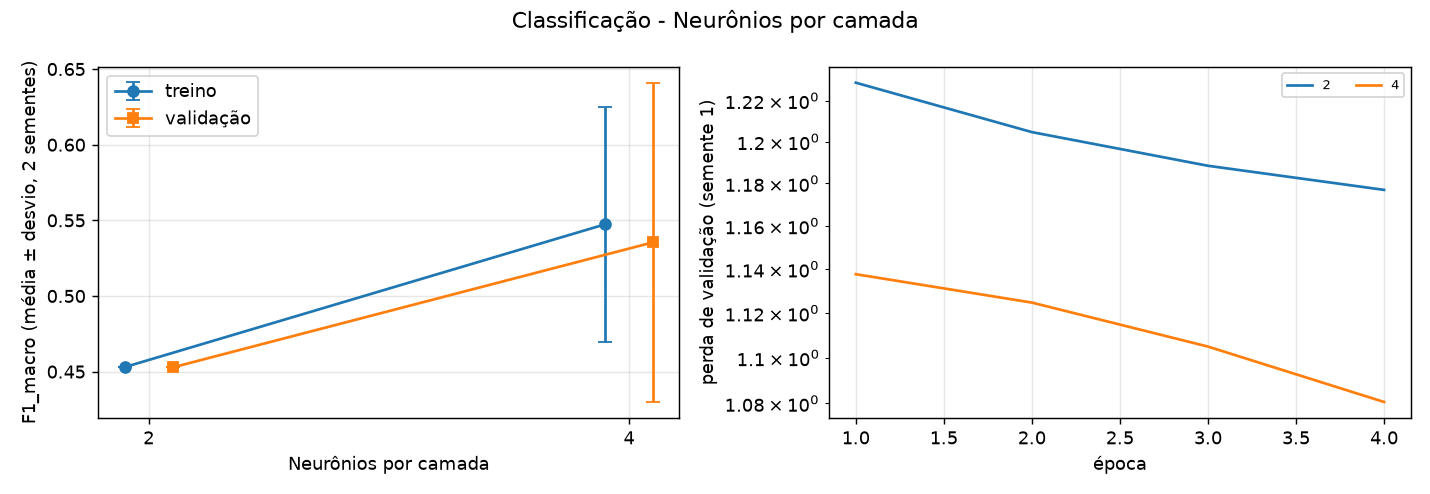
\includegraphics[width=0.95\linewidth]{hp_clf_neurons}\caption{Neurônios por camada -- classificação: métrica final por valor (esq.) e perda de validação por época (dir., semente 1).}\end{figure}
\begin{figure}[H]\centering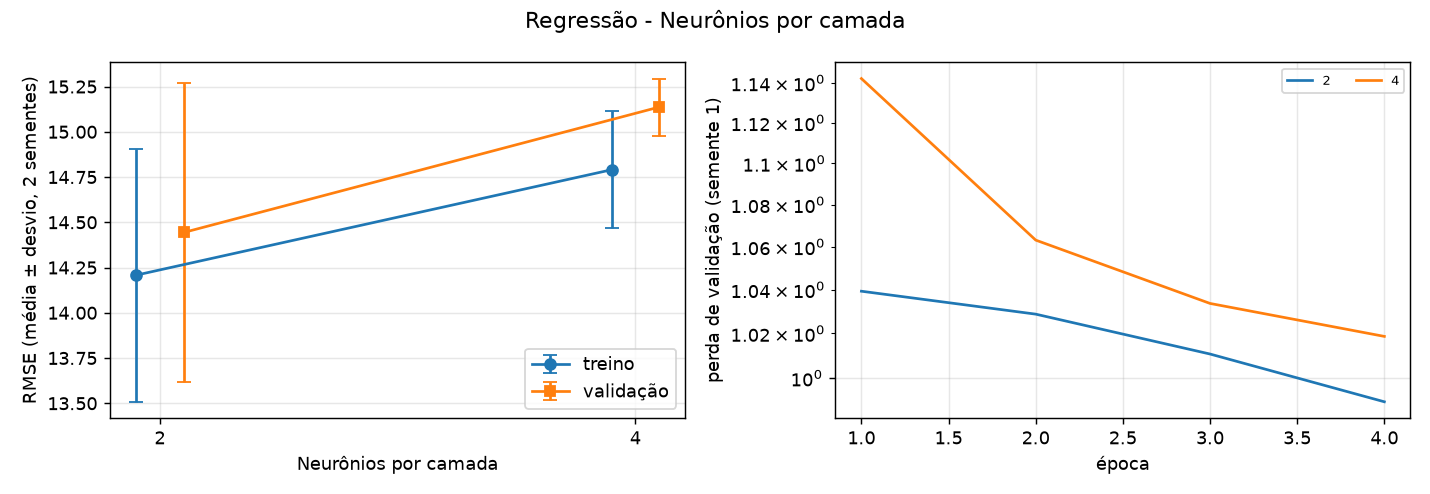
\includegraphics[width=0.95\linewidth]{hp_reg_neurons}\caption{Neurônios por camada -- regressão: métrica final por valor (esq.) e perda de validação por época (dir., semente 1).}\end{figure}
\paragraph{(a) Hipótese.} Poucos neurônios dão baixa capacidade (alto viés, underfitting); muitos neurônios reduzem o viés, mas aumentam a variância e o gap entre treino e validação.

\paragraph{(b) Evidência.} Na classificação, o melhor F1 macro de validação foi 0,535 $\pm$ 0,106 (4) e o pior 0,453 $\pm$ 0,000 (2); a diferença de 0,083 é menor que a soma dos desvios (0,106), logo o efeito está dentro do ruído entre sementes e não deve ser tratado como real. O gap variou de 0,000 (2) a 0,012 (4). A melhor época média foi de 4 (2) a 4 (2), e o tempo médio de treino de 0,3 s a 0,3 s. Na regressão, o melhor RMSE (mmHg) de validação foi 14,444 $\pm$ 0,827 (2) e o pior 15,137 $\pm$ 0,158 (4); a diferença de 0,693 é menor que a soma dos desvios (0,984), logo o efeito está dentro do ruído entre sementes e não deve ser tratado como real. O gap variou de 0,236 (2) a 0,346 (4). A melhor época média foi de 4 (2) a 4 (2), e o tempo médio de treino de 0,2 s a 0,2 s.

\paragraph{(c) Mecanismo.} O número de parâmetros cresce aproximadamente com o quadrado dos neurônios por camada; mais parâmetros permitem memorizar ruído do treino (variância), o que aparece como aumento do gap. Com sinal fraco (como neste conjunto sintético), a capacidade extra rende pouco na validação.
% REVISAR: relacione o mecanismo com as curvas acima.

\paragraph{(d) Conclusão prática.} Na classificação, os valores estatisticamente empatados com o melhor (4) foram: 2, 4. Com 2 neurônios o diagnóstico foi \emph{underfitting} (validação 0,453), e com 4 o gap foi 0,012 contra 0,000 com 2: a hipótese de que mais capacidade abre o gap se confirmou neste dataset. Na regressão, os valores estatisticamente empatados com o melhor (2) foram: 2, 4. Com 2 neurônios o diagnóstico foi \emph{bem ajustado} (validação 14,444), e com 4 o gap foi 0,346 contra 0,236 com 2: a hipótese de que mais capacidade abre o gap se confirmou neste dataset.
% REVISAR

\subsection{Camadas ocultas}
Valores testados: 1, 2.

\begin{table}[H]\centering\scriptsize\resizebox{\ifdim\width>\linewidth\linewidth\else\width\fi}{!}{%
\begin{tabular}{lrrrrrrr}\toprule
valor & parâm. & F1 macro treino & F1 macro validação & gap & época parada & tempo (s) & diagnóstico \\\midrule
1 & 2081 & 0,610 $\pm$ 0,019 & 0,577 $\pm$ 0,018 & 0,033 & 3,5 & 0,2 & bem ajustado \\
2 & 3137 & 0,622 $\pm$ 0,011 & 0,595 $\pm$ 0,013 & 0,027 & 3,0 & 0,3 & bem ajustado \\
\bottomrule\end{tabular}}
\caption{Camadas ocultas -- classificação (média $\pm$ desvio entre 2 sementes; gap = treino $-$ validação).}\label{tab:clf_layers}\end{table}
\begin{table}[H]\centering\scriptsize\resizebox{\ifdim\width>\linewidth\linewidth\else\width\fi}{!}{%
\begin{tabular}{lrrrrrrr}\toprule
valor & parâm. & RMSE (mmHg) treino & RMSE (mmHg) validação & gap & época parada & tempo (s) & diagnóstico \\\midrule
1 & 2209 & 13,280 $\pm$ 0,209 & 13,978 $\pm$ 0,038 & 0,698 & 3,0 & 0,2 & bem ajustado \\
2 & 3265 & 13,207 $\pm$ 0,069 & 13,920 $\pm$ 0,020 & 0,714 & 3,0 & 0,3 & bem ajustado \\
\bottomrule\end{tabular}}
\caption{Camadas ocultas -- regressão (média $\pm$ desvio entre 2 sementes; gap = treino $-$ validação em erro: validação $-$ treino).}\label{tab:reg_layers}\end{table}
\begin{figure}[H]\centering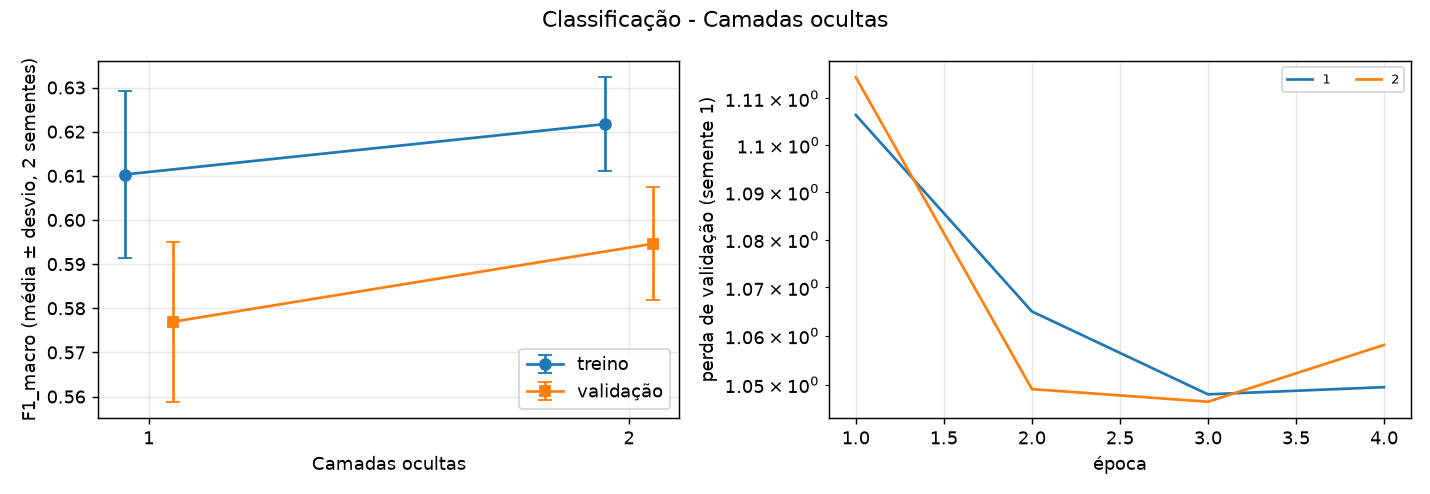
\includegraphics[width=0.95\linewidth]{hp_clf_layers}\caption{Camadas ocultas -- classificação: métrica final por valor (esq.) e perda de validação por época (dir., semente 1).}\end{figure}
\begin{figure}[H]\centering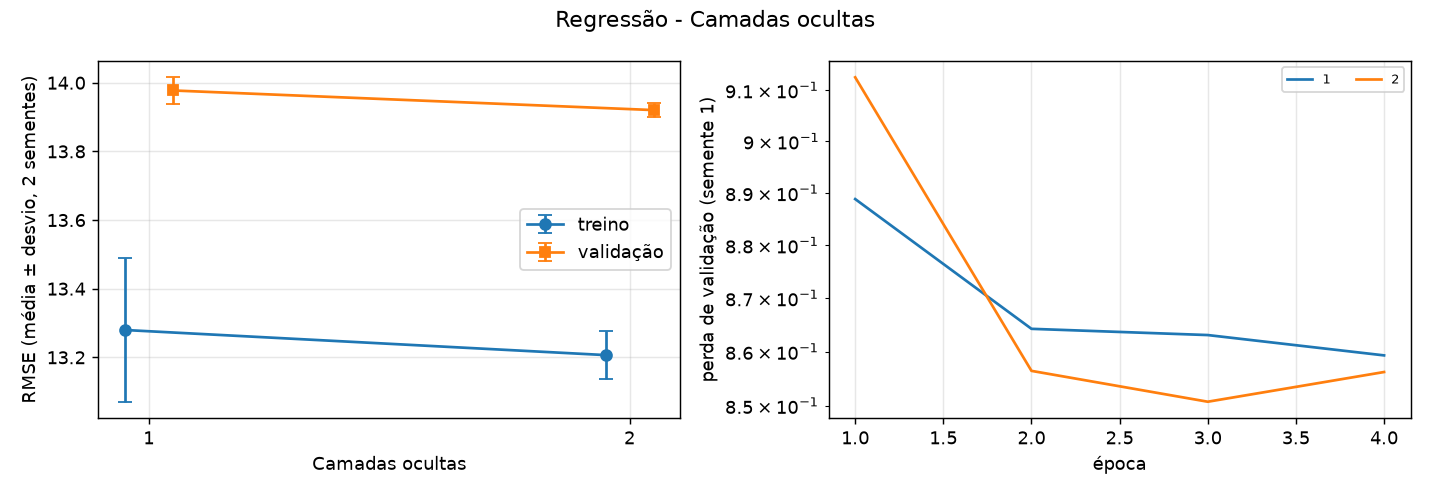
\includegraphics[width=0.95\linewidth]{hp_reg_layers}\caption{Camadas ocultas -- regressão: métrica final por valor (esq.) e perda de validação por época (dir., semente 1).}\end{figure}
\paragraph{(a) Hipótese.} Mais camadas aumentam a capacidade e o número de parâmetros, mas tornam a otimização mais difícil (gradientes atravessam mais derivadas encadeadas); para dados tabulares com sinal fraco, redes rasas devem bastar.

\paragraph{(b) Evidência.} Na classificação, o melhor F1 macro de validação foi 0,595 $\pm$ 0,013 (2) e o pior 0,577 $\pm$ 0,018 (1); a diferença de 0,018 é menor que a soma dos desvios (0,031), logo o efeito está dentro do ruído entre sementes e não deve ser tratado como real. O gap variou de 0,027 (2) a 0,033 (1). A melhor época média foi de 3 (2) a 4 (1), e o tempo médio de treino de 0,2 s a 0,3 s. Na regressão, o melhor RMSE (mmHg) de validação foi 13,920 $\pm$ 0,020 (2) e o pior 13,978 $\pm$ 0,038 (1); a diferença de 0,057 é menor que a soma dos desvios (0,058), logo o efeito está dentro do ruído entre sementes e não deve ser tratado como real. O gap variou de 0,698 (1) a 0,714 (2). A melhor época média foi de 3 (1) a 3 (1), e o tempo médio de treino de 0,2 s a 0,3 s.

\paragraph{(c) Mecanismo.} Cada camada a mais compõe uma transformação não linear; o gradiente das primeiras camadas é produto de várias derivadas, podendo encolher. O early stopping limita o overfitting, mas não compensa a otimização mais difícil.
% REVISAR: relacione o mecanismo com as curvas acima.

\paragraph{(d) Conclusão prática.} Na classificação, os valores estatisticamente empatados com o melhor (2) foram: 1, 2. Passar de 1 para 2 camada(s) multiplicou os parâmetros de 2081 para 3137 e não piorou a validação (0,577 $\to$ 0,595). Na regressão, os valores estatisticamente empatados com o melhor (2) foram: 1, 2. Passar de 1 para 2 camada(s) multiplicou os parâmetros de 2209 para 3265 e não piorou a validação (13,978 $\to$ 13,920).
% REVISAR

\subsection{Função de ativação}
Valores testados: ReLU, LeakyReLU.

\begin{table}[H]\centering\scriptsize\resizebox{\ifdim\width>\linewidth\linewidth\else\width\fi}{!}{%
\begin{tabular}{lrrrrrrr}\toprule
valor & parâm. & F1 macro treino & F1 macro validação & gap & época parada & tempo (s) & diagnóstico \\\midrule
ReLU & 3137 & 0,622 $\pm$ 0,011 & 0,595 $\pm$ 0,013 & 0,027 & 3,0 & 0,3 & bem ajustado \\
LeakyReLU & 3137 & 0,622 $\pm$ 0,008 & 0,593 $\pm$ 0,015 & 0,029 & 3,0 & 0,3 & bem ajustado \\
\bottomrule\end{tabular}}
\caption{Função de ativação -- classificação (média $\pm$ desvio entre 2 sementes; gap = treino $-$ validação).}\label{tab:clf_activation}\end{table}
\begin{table}[H]\centering\scriptsize\resizebox{\ifdim\width>\linewidth\linewidth\else\width\fi}{!}{%
\begin{tabular}{lrrrrrrr}\toprule
valor & parâm. & RMSE (mmHg) treino & RMSE (mmHg) validação & gap & época parada & tempo (s) & diagnóstico \\\midrule
ReLU & 3265 & 13,207 $\pm$ 0,069 & 13,920 $\pm$ 0,020 & 0,714 & 3,0 & 0,3 & bem ajustado \\
LeakyReLU & 3265 & 13,210 $\pm$ 0,064 & 13,908 $\pm$ 0,022 & 0,698 & 3,0 & 0,3 & bem ajustado \\
\bottomrule\end{tabular}}
\caption{Função de ativação -- regressão (média $\pm$ desvio entre 2 sementes; gap = treino $-$ validação em erro: validação $-$ treino).}\label{tab:reg_activation}\end{table}
\begin{figure}[H]\centering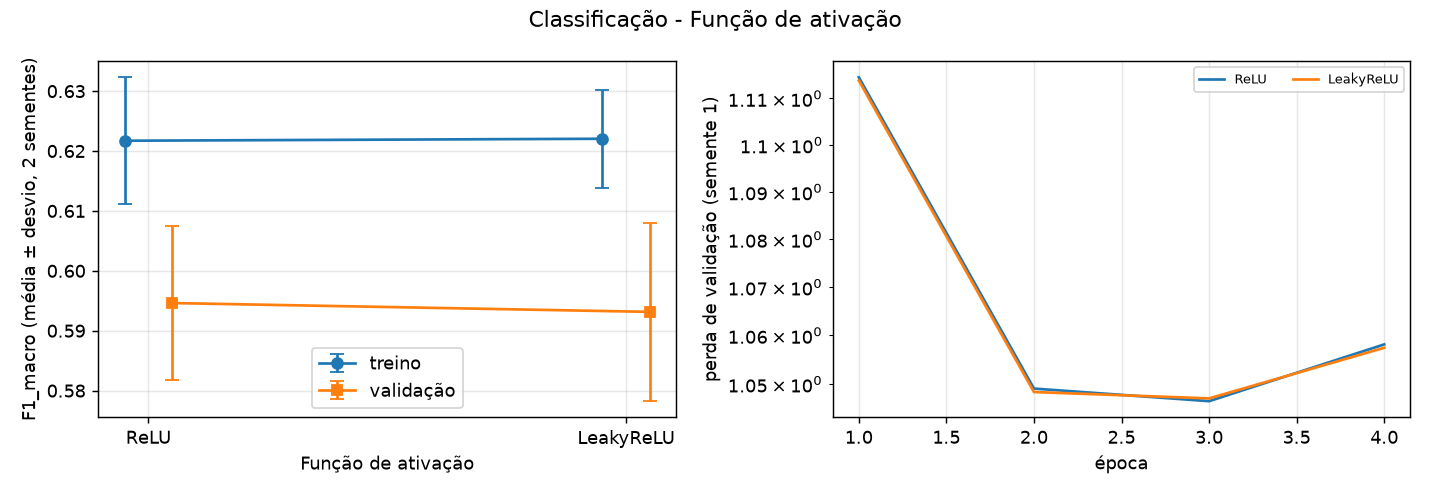
\includegraphics[width=0.95\linewidth]{hp_clf_activation}\caption{Função de ativação -- classificação: métrica final por valor (esq.) e perda de validação por época (dir., semente 1).}\end{figure}
\begin{figure}[H]\centering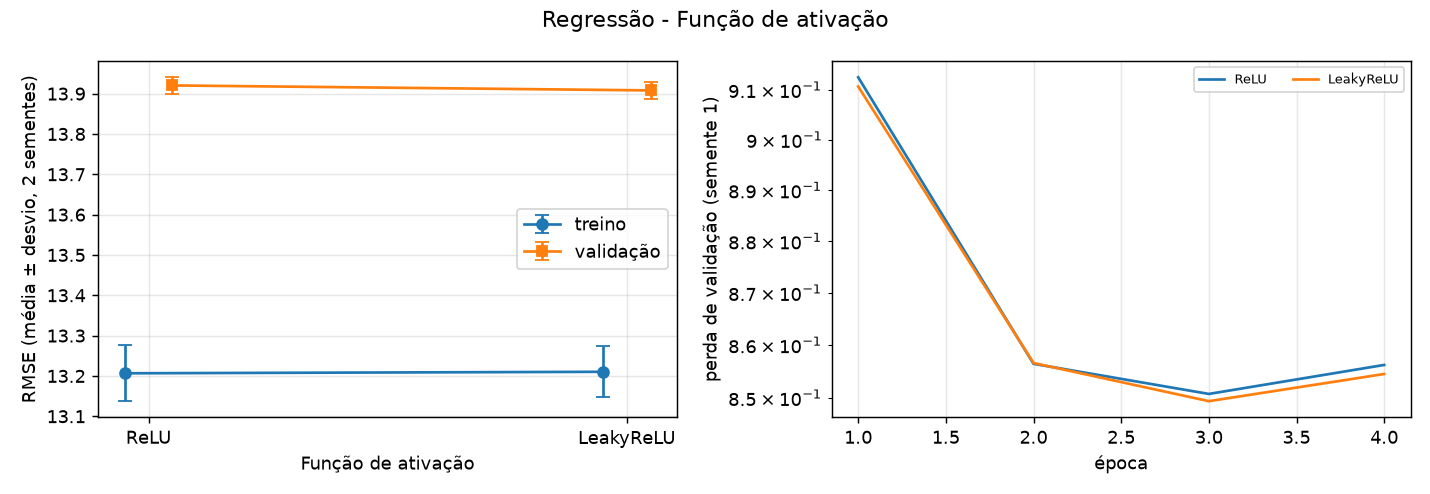
\includegraphics[width=0.95\linewidth]{hp_reg_activation}\caption{Função de ativação -- regressão: métrica final por valor (esq.) e perda de validação por época (dir., semente 1).}\end{figure}
\paragraph{(a) Hipótese.} Sigmoid e Tanh saturam (derivada próxima de zero para entradas grandes) e devem convergir mais devagar; ReLU, LeakyReLU e GELU não saturam para entradas positivas.

\paragraph{(b) Evidência.} Na classificação, o melhor F1 macro de validação foi 0,595 $\pm$ 0,013 (ReLU) e o pior 0,593 $\pm$ 0,015 (LeakyReLU); a diferença de 0,001 é menor que a soma dos desvios (0,028), logo o efeito está dentro do ruído entre sementes e não deve ser tratado como real. O gap variou de 0,027 (ReLU) a 0,029 (LeakyReLU). A melhor época média foi de 3 (ReLU) a 3 (ReLU), e o tempo médio de treino de 0,3 s a 0,3 s. Na regressão, o melhor RMSE (mmHg) de validação foi 13,908 $\pm$ 0,022 (LeakyReLU) e o pior 13,920 $\pm$ 0,020 (ReLU); a diferença de 0,012 é menor que a soma dos desvios (0,042), logo o efeito está dentro do ruído entre sementes e não deve ser tratado como real. O gap variou de 0,698 (LeakyReLU) a 0,714 (ReLU). A melhor época média foi de 3 (ReLU) a 3 (ReLU), e o tempo médio de treino de 0,3 s a 0,3 s.

\paragraph{(c) Mecanismo.} A derivada da sigmoide é no máximo 0,25 e a da tanh no máximo 1, ambas tendendo a zero na saturação; ao multiplicar essas derivadas entre camadas, o gradiente enfraquece. A ReLU tem derivada 1 para entradas positivas (mas zero para negativas, o que pode \emph{matar} neurônios), e a LeakyReLU/GELU mantêm gradiente também para entradas negativas.
% REVISAR: relacione o mecanismo com as curvas acima.

\paragraph{(d) Conclusão prática.} Na classificação, os valores estatisticamente empatados com o melhor (ReLU) foram: ReLU, LeakyReLU.  Na regressão, os valores estatisticamente empatados com o melhor (LeakyReLU) foram: ReLU, LeakyReLU. 
% REVISAR

\subsection{Otimizador}
Valores testados: SGD, SGD\_momentum.

\begin{table}[H]\centering\scriptsize\resizebox{\ifdim\width>\linewidth\linewidth\else\width\fi}{!}{%
\begin{tabular}{lrrrrrrr}\toprule
valor & parâm. & F1 macro treino & F1 macro validação & gap & época parada & tempo (s) & diagnóstico \\\midrule
SGD & 3137 & 0,418 $\pm$ 0,138 & 0,417 $\pm$ 0,145 & 0,001 & 4,0 & 0,2 & underfitting \\
SGD\_momentum & 3137 & 0,529 $\pm$ 0,030 & 0,534 $\pm$ 0,032 & -0,005 & 4,0 & 0,2 & bem ajustado \\
\bottomrule\end{tabular}}
\caption{Otimizador -- classificação (média $\pm$ desvio entre 2 sementes; gap = treino $-$ validação).}\label{tab:clf_optimizer}\end{table}
\begin{table}[H]\centering\scriptsize\resizebox{\ifdim\width>\linewidth\linewidth\else\width\fi}{!}{%
\begin{tabular}{lrrrrrrr}\toprule
valor & parâm. & RMSE (mmHg) treino & RMSE (mmHg) validação & gap & época parada & tempo (s) & diagnóstico \\\midrule
SGD & 3265 & 15,109 $\pm$ 0,005 & 15,360 $\pm$ 0,025 & 0,251 & 4,0 & 0,2 & underfitting \\
SGD\_momentum & 3265 & 13,889 $\pm$ 0,137 & 14,183 $\pm$ 0,077 & 0,294 & 4,0 & 0,2 & bem ajustado \\
\bottomrule\end{tabular}}
\caption{Otimizador -- regressão (média $\pm$ desvio entre 2 sementes; gap = treino $-$ validação em erro: validação $-$ treino).}\label{tab:reg_optimizer}\end{table}
\begin{figure}[H]\centering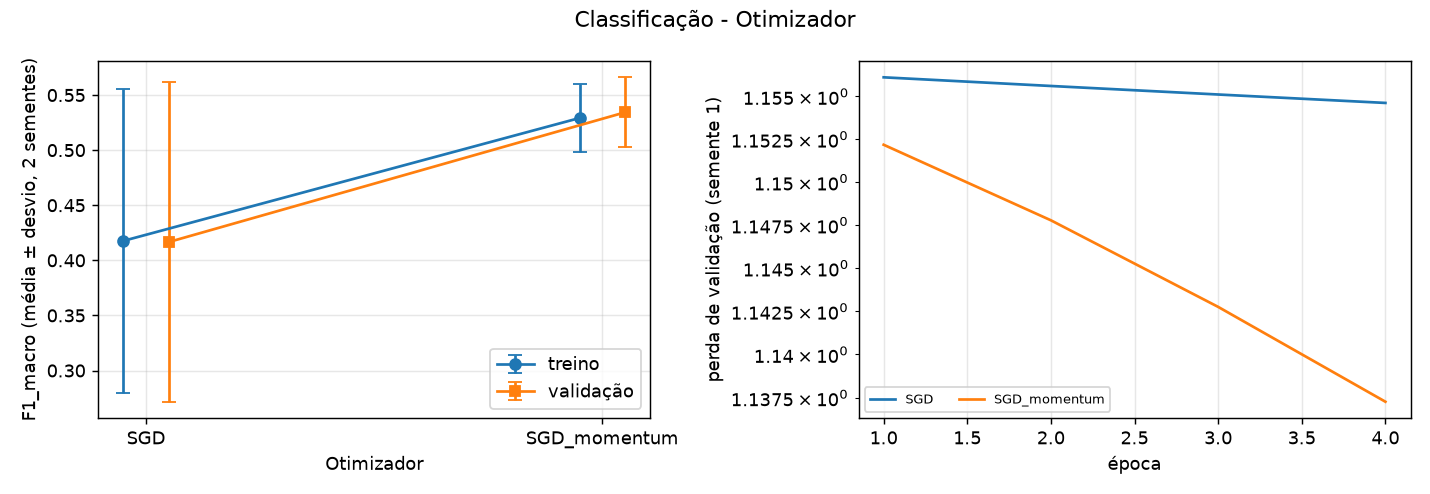
\includegraphics[width=0.95\linewidth]{hp_clf_optimizer}\caption{Otimizador -- classificação: métrica final por valor (esq.) e perda de validação por época (dir., semente 1).}\end{figure}
\begin{figure}[H]\centering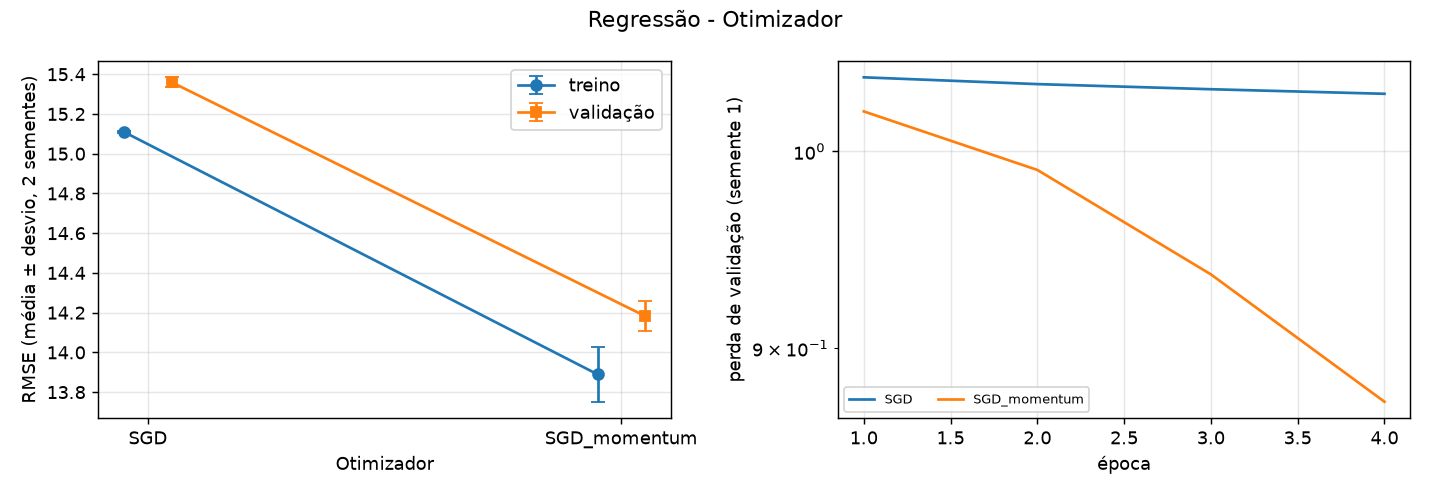
\includegraphics[width=0.95\linewidth]{hp_reg_optimizer}\caption{Otimizador -- regressão: métrica final por valor (esq.) e perda de validação por época (dir., semente 1).}\end{figure}
\paragraph{(a) Hipótese.} SGD sem momento com $\eta=10^{-3}$ deve convergir lentamente; momento acelera a descida em direções consistentes, e RMSprop/Adam/AdamW adaptam o passo por parâmetro e convergem mais rápido.

\paragraph{(b) Evidência.} Na classificação, o melhor F1 macro de validação foi 0,534 $\pm$ 0,032 (SGD\_momentum) e o pior 0,417 $\pm$ 0,145 (SGD); a diferença de 0,118 é menor que a soma dos desvios (0,177), logo o efeito está dentro do ruído entre sementes e não deve ser tratado como real. O gap variou de -0,005 (SGD\_momentum) a 0,001 (SGD). A melhor época média foi de 4 (SGD) a 4 (SGD), e o tempo médio de treino de 0,2 s a 0,2 s. Na regressão, o melhor RMSE (mmHg) de validação foi 14,183 $\pm$ 0,077 (SGD\_momentum) e o pior 15,360 $\pm$ 0,025 (SGD); a diferença de 1,176 é maior que a soma dos desvios (0,101), logo o efeito é real. O gap variou de 0,251 (SGD) a 0,294 (SGD\_momentum). A melhor época média foi de 4 (SGD) a 4 (SGD), e o tempo médio de treino de 0,2 s a 0,2 s.

\paragraph{(c) Mecanismo.} O SGD usa o mesmo passo para todos os parâmetros; o momento acumula uma média dos gradientes anteriores; RMSprop e Adam dividem o passo pela raiz da média dos gradientes ao quadrado, adaptando-o a cada parâmetro; o AdamW aplica o decaimento de pesos de forma desacoplada (aqui com o padrão do PyTorch, 0,01).
% REVISAR: relacione o mecanismo com as curvas acima.

\paragraph{(d) Conclusão prática.} Na classificação, os valores estatisticamente empatados com o melhor (SGD\_momentum) foram: SGD, SGD\_momentum.  Na regressão, os valores estatisticamente empatados com o melhor (SGD\_momentum) foram: SGD\_momentum. 
% REVISAR

\subsection{Taxa de aprendizado}
Valores testados: 0,0001, 0,001.

\begin{table}[H]\centering\scriptsize\resizebox{\ifdim\width>\linewidth\linewidth\else\width\fi}{!}{%
\begin{tabular}{lrrrrrrr}\toprule
valor & parâm. & F1 macro treino & F1 macro validação & gap & época parada & tempo (s) & diagnóstico \\\midrule
0,0001 & 3137 & 0,528 $\pm$ 0,077 & 0,526 $\pm$ 0,080 & 0,002 & 4,0 & 0,3 & bem ajustado \\
0,001 & 3137 & 0,622 $\pm$ 0,011 & 0,595 $\pm$ 0,013 & 0,027 & 3,0 & 0,3 & bem ajustado \\
\bottomrule\end{tabular}}
\caption{Taxa de aprendizado -- classificação (média $\pm$ desvio entre 2 sementes; gap = treino $-$ validação).}\label{tab:clf_lr}\end{table}
\begin{table}[H]\centering\scriptsize\resizebox{\ifdim\width>\linewidth\linewidth\else\width\fi}{!}{%
\begin{tabular}{lrrrrrrr}\toprule
valor & parâm. & RMSE (mmHg) treino & RMSE (mmHg) validação & gap & época parada & tempo (s) & diagnóstico \\\midrule
0,0001 & 3265 & 14,794 $\pm$ 0,043 & 15,104 $\pm$ 0,026 & 0,310 & 4,0 & 0,3 & underfitting \\
0,001 & 3265 & 13,207 $\pm$ 0,069 & 13,920 $\pm$ 0,020 & 0,714 & 3,0 & 0,3 & bem ajustado \\
\bottomrule\end{tabular}}
\caption{Taxa de aprendizado -- regressão (média $\pm$ desvio entre 2 sementes; gap = treino $-$ validação em erro: validação $-$ treino).}\label{tab:reg_lr}\end{table}
\begin{figure}[H]\centering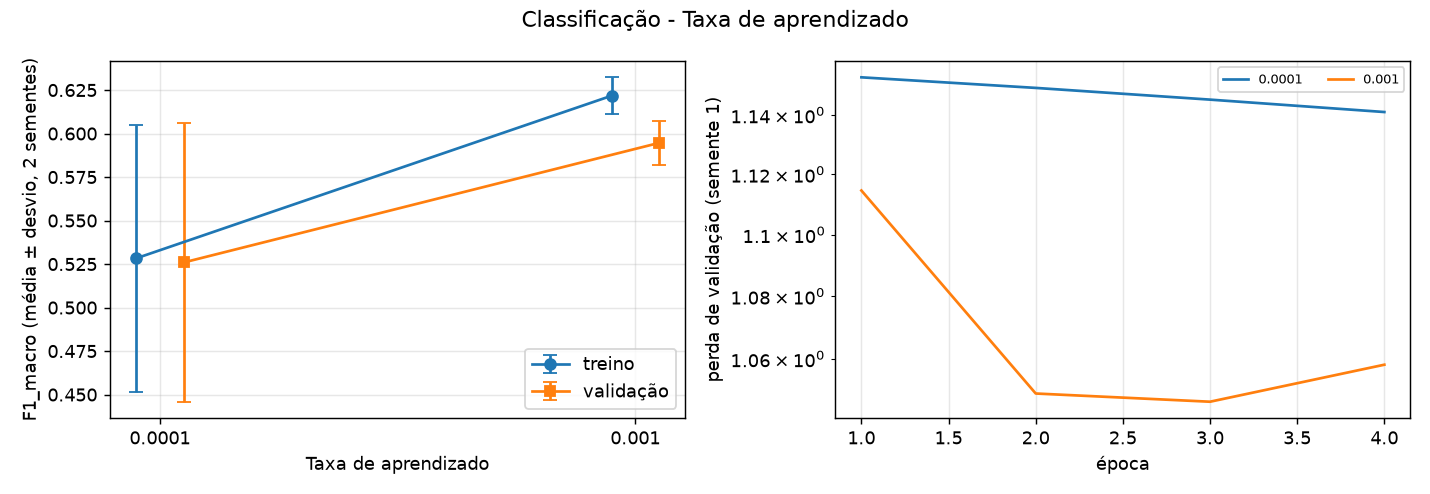
\includegraphics[width=0.95\linewidth]{hp_clf_lr}\caption{Taxa de aprendizado -- classificação: métrica final por valor (esq.) e perda de validação por época (dir., semente 1).}\end{figure}
\begin{figure}[H]\centering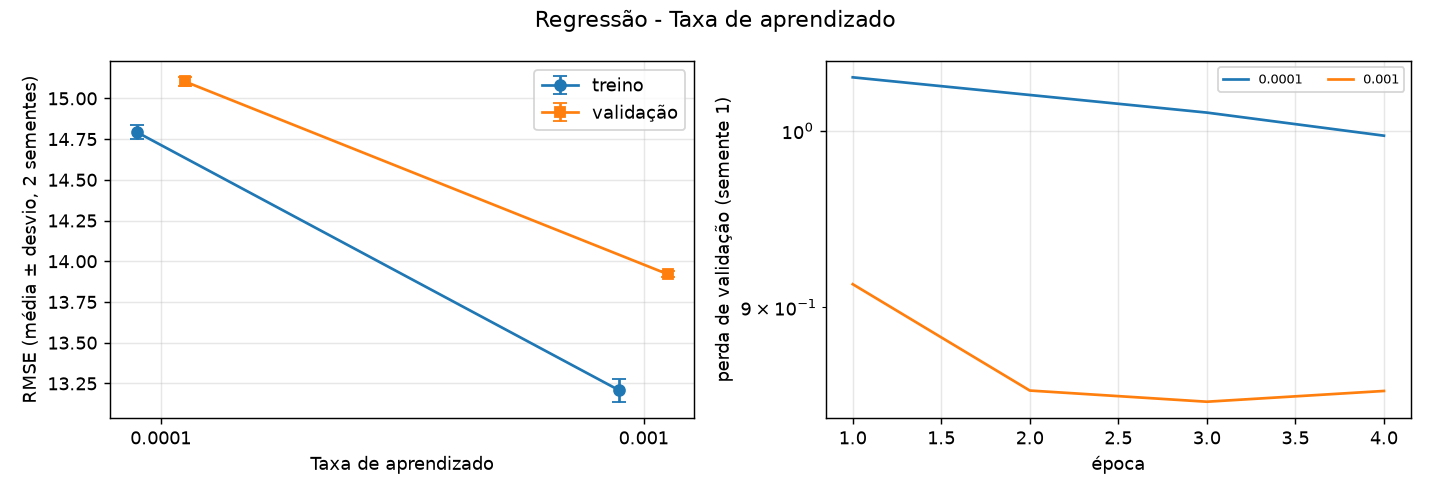
\includegraphics[width=0.95\linewidth]{hp_reg_lr}\caption{Taxa de aprendizado -- regressão: métrica final por valor (esq.) e perda de validação por época (dir., semente 1).}\end{figure}
\paragraph{(a) Hipótese.} $\eta$ muito alto faz a atualização $\theta \leftarrow \theta - \eta\nabla_\theta L$ ultrapassar o mínimo (oscilação ou divergência); $\eta$ muito baixo faz a perda cair devagar e o treino pode terminar antes de convergir.

\paragraph{(b) Evidência.} Na classificação, o melhor F1 macro de validação foi 0,595 $\pm$ 0,013 (0,001) e o pior 0,526 $\pm$ 0,080 (0,0001); a diferença de 0,069 é menor que a soma dos desvios (0,093), logo o efeito está dentro do ruído entre sementes e não deve ser tratado como real. O gap variou de 0,002 (0,0001) a 0,027 (0,001). A melhor época média foi de 3 (0,001) a 4 (0,0001), e o tempo médio de treino de 0,3 s a 0,3 s. Na regressão, o melhor RMSE (mmHg) de validação foi 13,920 $\pm$ 0,020 (0,001) e o pior 15,104 $\pm$ 0,026 (0,0001); a diferença de 1,183 é maior que a soma dos desvios (0,046), logo o efeito é real. O gap variou de 0,310 (0,0001) a 0,714 (0,001). A melhor época média foi de 3 (0,001) a 4 (0,0001), e o tempo médio de treino de 0,3 s a 0,3 s.

\paragraph{(c) Mecanismo.} O tamanho do passo controla o equilíbrio entre velocidade e estabilidade: passos grandes amplificam o erro de cada atualização (a perda explode e vira NaN), passos pequenos precisam de muitas épocas e o limite de épocas é atingido antes da convergência.
% REVISAR: relacione o mecanismo com as curvas acima.

\paragraph{(d) Conclusão prática.} Na classificação, os valores estatisticamente empatados com o melhor (0,001) foram: 0,0001, 0,001. Com $\eta$ = 0,0001 o treino rodou em média 4 de 4 épocas (atingiu o limite: convergência lenta); com $\eta$ = 0,001 não houve divergência, mas a validação foi 0,595. Na regressão, os valores estatisticamente empatados com o melhor (0,001) foram: 0,001. Com $\eta$ = 0,0001 o treino rodou em média 4 de 4 épocas (atingiu o limite: convergência lenta); com $\eta$ = 0,001 não houve divergência, mas a validação foi 13,920.
% REVISAR

\subsection{Tamanho do batch}
Valores testados: 8, 32.

\begin{table}[H]\centering\scriptsize\resizebox{\ifdim\width>\linewidth\linewidth\else\width\fi}{!}{%
\begin{tabular}{lrrrrrrr}\toprule
valor & parâm. & F1 macro treino & F1 macro validação & gap & época parada & tempo (s) & diagnóstico \\\midrule
8 & 3137 & 0,619 $\pm$ 0,013 & 0,582 $\pm$ 0,006 & 0,037 & 2,0 & 0,9 & bem ajustado \\
32 & 3137 & 0,622 $\pm$ 0,011 & 0,595 $\pm$ 0,013 & 0,027 & 3,0 & 0,3 & bem ajustado \\
\bottomrule\end{tabular}}
\caption{Tamanho do batch -- classificação (média $\pm$ desvio entre 2 sementes; gap = treino $-$ validação).}\label{tab:clf_batch}\end{table}
\begin{table}[H]\centering\scriptsize\resizebox{\ifdim\width>\linewidth\linewidth\else\width\fi}{!}{%
\begin{tabular}{lrrrrrrr}\toprule
valor & parâm. & RMSE (mmHg) treino & RMSE (mmHg) validação & gap & época parada & tempo (s) & diagnóstico \\\midrule
8 & 3265 & 13,354 $\pm$ 0,261 & 13,874 $\pm$ 0,018 & 0,520 & 1,5 & 0,8 & bem ajustado \\
32 & 3265 & 13,207 $\pm$ 0,069 & 13,920 $\pm$ 0,020 & 0,714 & 3,0 & 0,3 & bem ajustado \\
\bottomrule\end{tabular}}
\caption{Tamanho do batch -- regressão (média $\pm$ desvio entre 2 sementes; gap = treino $-$ validação em erro: validação $-$ treino).}\label{tab:reg_batch}\end{table}
\begin{figure}[H]\centering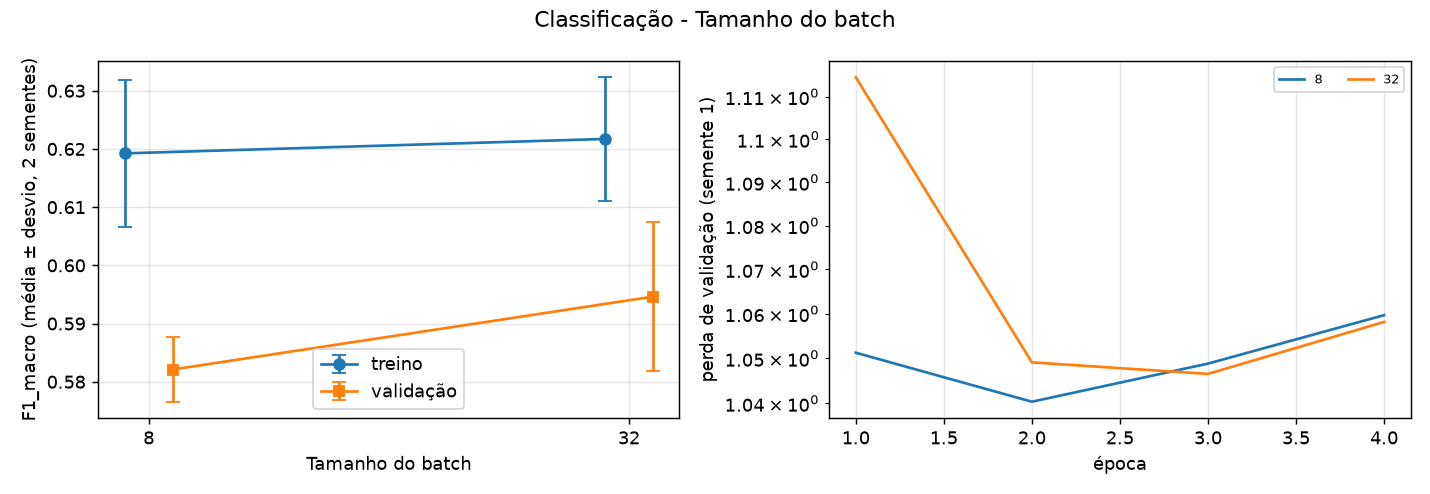
\includegraphics[width=0.95\linewidth]{hp_clf_batch}\caption{Tamanho do batch -- classificação: métrica final por valor (esq.) e perda de validação por época (dir., semente 1).}\end{figure}
\begin{figure}[H]\centering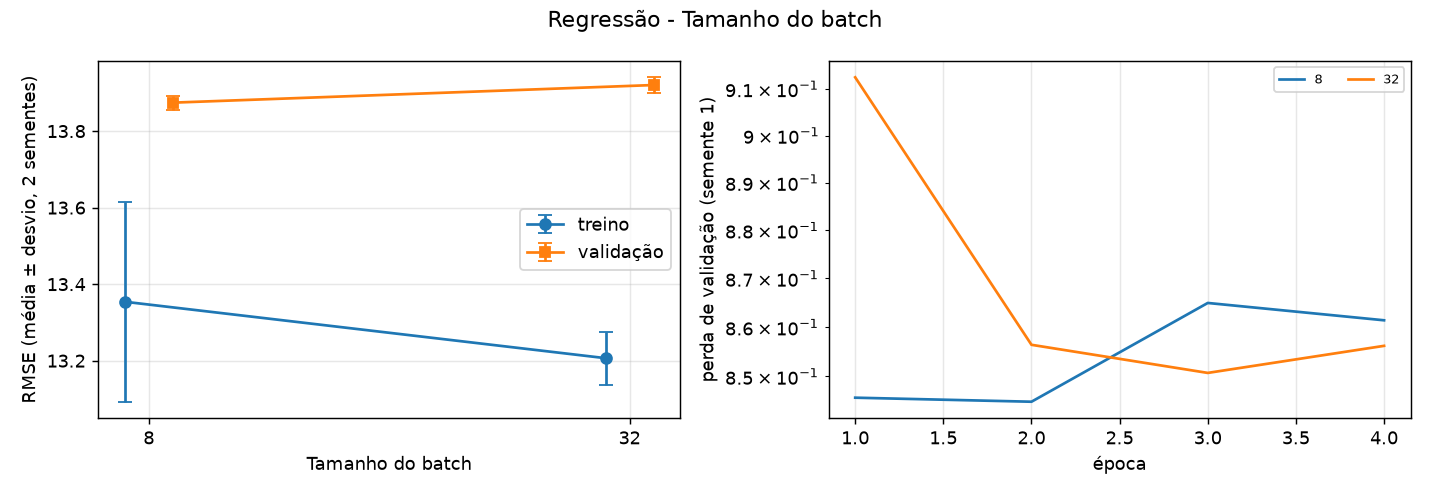
\includegraphics[width=0.95\linewidth]{hp_reg_batch}\caption{Tamanho do batch -- regressão: métrica final por valor (esq.) e perda de validação por época (dir., semente 1).}\end{figure}
\paragraph{(a) Hipótese.} Batches pequenos dão gradientes ruidosos e muitas atualizações por época (mais tempo por época, algum efeito regularizador); batches grandes dão gradientes estáveis, mas poucas atualizações por época, exigindo mais épocas ou $\eta$ maior.

\paragraph{(b) Evidência.} Na classificação, o melhor F1 macro de validação foi 0,595 $\pm$ 0,013 (32) e o pior 0,582 $\pm$ 0,006 (8); a diferença de 0,013 é menor que a soma dos desvios (0,018), logo o efeito está dentro do ruído entre sementes e não deve ser tratado como real. O gap variou de 0,027 (32) a 0,037 (8). A melhor época média foi de 2 (8) a 3 (32), e o tempo médio de treino de 0,3 s a 0,9 s. Na regressão, o melhor RMSE (mmHg) de validação foi 13,874 $\pm$ 0,018 (8) e o pior 13,920 $\pm$ 0,020 (32); a diferença de 0,046 é maior que a soma dos desvios (0,038), logo o efeito é real. O gap variou de 0,520 (8) a 0,714 (32). A melhor época média foi de 2 (8) a 3 (32), e o tempo médio de treino de 0,3 s a 0,8 s.

\paragraph{(c) Mecanismo.} Com $n$ amostras de treino e batch $B$, há $\lceil n/B \rceil$ atualizações por época: o batch pequeno faz mais atualizações (mais tempo por época, pois cada passo tem custo fixo) com gradiente ruidoso; o batch grande aproveita melhor o paralelismo, mas dá poucos passos por época.
% REVISAR: relacione o mecanismo com as curvas acima.

\paragraph{(d) Conclusão prática.} Na classificação, os valores estatisticamente empatados com o melhor (32) foram: 8, 32. Com batch 8 o treino levou 0,9 s (muitas atualizações por época) e com 32 0,3 s; a validação foi 0,582 e 0,595, respectivamente, e a melhor época passou de 2 para 3. Na regressão, os valores estatisticamente empatados com o melhor (8) foram: 8. Com batch 8 o treino levou 0,8 s (muitas atualizações por época) e com 32 0,3 s; a validação foi 13,874 e 13,920, respectivamente, e a melhor época passou de 2 para 3.
% REVISAR

\subsection{Weight decay (L2)}
Valores testados: 0, 1e-05 (opcional).

\begin{table}[H]\centering\scriptsize\resizebox{\ifdim\width>\linewidth\linewidth\else\width\fi}{!}{%
\begin{tabular}{lrrrrrrr}\toprule
valor & parâm. & F1 macro treino & F1 macro validação & gap & época parada & tempo (s) & diagnóstico \\\midrule
0 & 3137 & 0,622 $\pm$ 0,011 & 0,595 $\pm$ 0,013 & 0,027 & 3,0 & 0,3 & bem ajustado \\
1e-05 & 3137 & 0,622 $\pm$ 0,009 & 0,594 $\pm$ 0,012 & 0,028 & 3,0 & 0,3 & bem ajustado \\
\bottomrule\end{tabular}}
\caption{Weight decay (L2) -- classificação (média $\pm$ desvio entre 2 sementes; gap = treino $-$ validação).}\label{tab:clf_weight_decay}\end{table}
\begin{table}[H]\centering\scriptsize\resizebox{\ifdim\width>\linewidth\linewidth\else\width\fi}{!}{%
\begin{tabular}{lrrrrrrr}\toprule
valor & parâm. & RMSE (mmHg) treino & RMSE (mmHg) validação & gap & época parada & tempo (s) & diagnóstico \\\midrule
0 & 3265 & 13,207 $\pm$ 0,069 & 13,920 $\pm$ 0,020 & 0,714 & 3,0 & 0,3 & bem ajustado \\
1e-05 & 3265 & 13,202 $\pm$ 0,070 & 13,916 $\pm$ 0,023 & 0,714 & 3,0 & 0,3 & bem ajustado \\
\bottomrule\end{tabular}}
\caption{Weight decay (L2) -- regressão (média $\pm$ desvio entre 2 sementes; gap = treino $-$ validação em erro: validação $-$ treino).}\label{tab:reg_weight_decay}\end{table}
\begin{figure}[H]\centering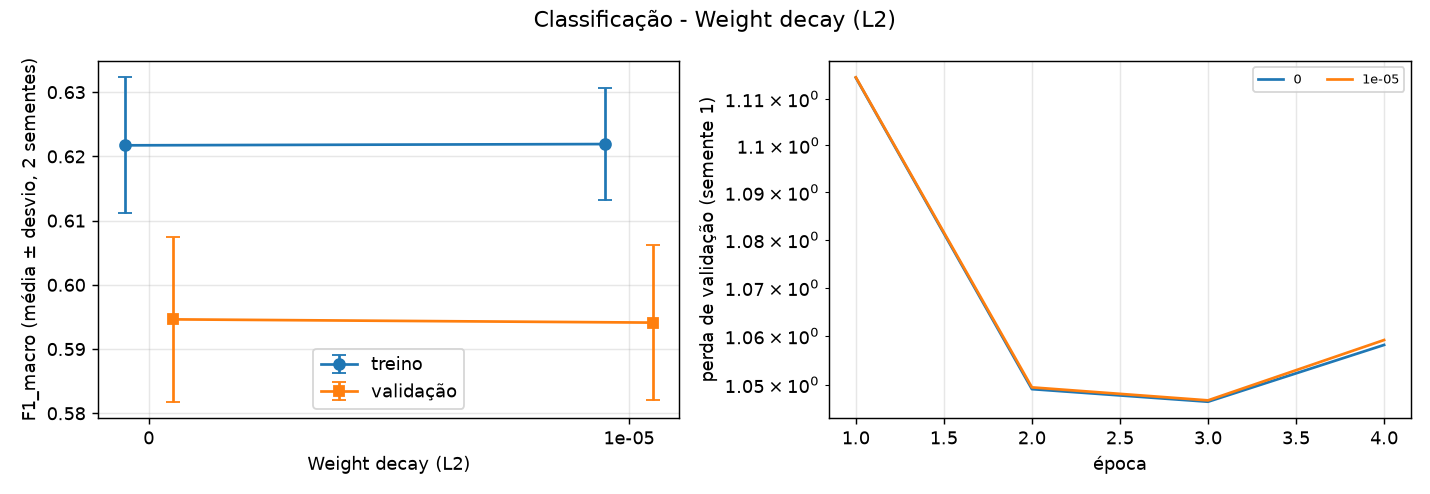
\includegraphics[width=0.95\linewidth]{hp_clf_weight_decay}\caption{Weight decay (L2) -- classificação: métrica final por valor (esq.) e perda de validação por época (dir., semente 1).}\end{figure}
\begin{figure}[H]\centering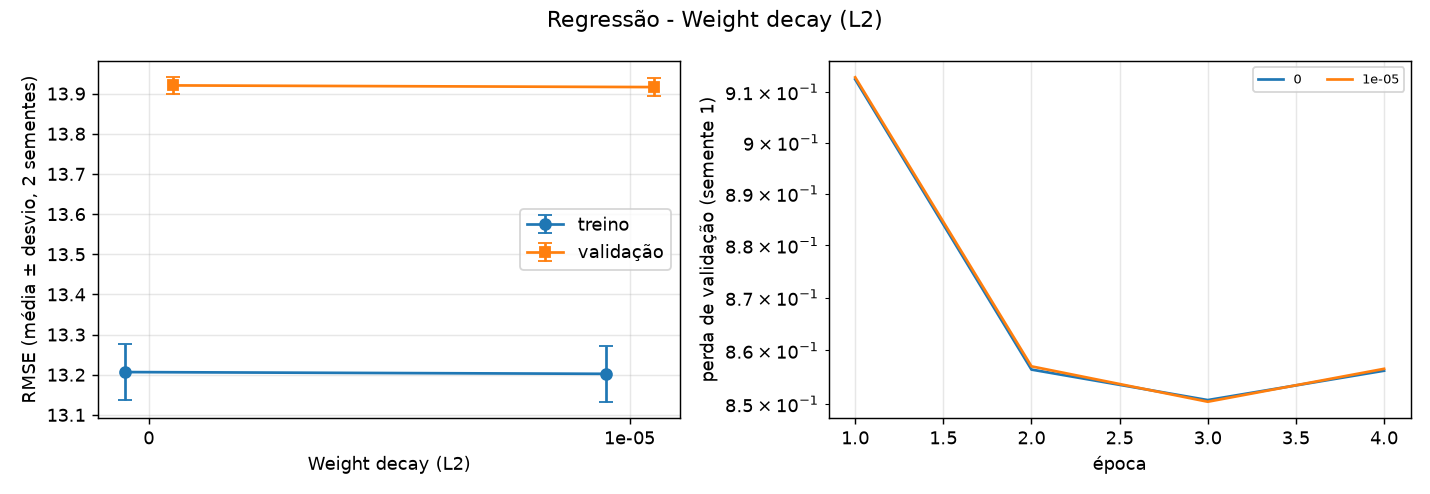
\includegraphics[width=0.95\linewidth]{hp_reg_weight_decay}\caption{Weight decay (L2) -- regressão: métrica final por valor (esq.) e perda de validação por época (dir., semente 1).}\end{figure}
\paragraph{(a) Hipótese.} A penalização L2 encolhe os pesos, reduz a variância e o gap; valores altos demais causam underfitting.

\paragraph{(b) Evidência.} Na classificação, o melhor F1 macro de validação foi 0,595 $\pm$ 0,013 (0) e o pior 0,594 $\pm$ 0,012 (1e-05); a diferença de 0,001 é menor que a soma dos desvios (0,025), logo o efeito está dentro do ruído entre sementes e não deve ser tratado como real. O gap variou de 0,027 (0) a 0,028 (1e-05). A melhor época média foi de 3 (0) a 3 (0), e o tempo médio de treino de 0,3 s a 0,3 s. Na regressão, o melhor RMSE (mmHg) de validação foi 13,916 $\pm$ 0,023 (1e-05) e o pior 13,920 $\pm$ 0,020 (0); a diferença de 0,004 é menor que a soma dos desvios (0,043), logo o efeito está dentro do ruído entre sementes e não deve ser tratado como real. O gap variou de 0,714 (0) a 0,714 (1e-05). A melhor época média foi de 3 (0) a 3 (0), e o tempo médio de treino de 0,3 s a 0,3 s.

\paragraph{(c) Mecanismo.} O termo $\lambda\lVert\theta\rVert^2$ soma $2\lambda\theta$ ao gradiente, puxando os pesos para zero e suavizando a função aprendida (menos variância, mais viés).
% REVISAR: relacione o mecanismo com as curvas acima.

\paragraph{(d) Conclusão prática.} Na classificação, os valores estatisticamente empatados com o melhor (0) foram: 0, 1e-05. Do menor (0) para o maior valor (1e-05), o desempenho de treino foi de 0,622 para 0,622 e o gap de 0,027 para 0,028: a hipótese de redução da variância não se confirmou (diagnóstico com o maior valor: bem ajustado). Na regressão, os valores estatisticamente empatados com o melhor (1e-05) foram: 0, 1e-05. Do menor (0) para o maior valor (1e-05), o desempenho de treino foi de 13,207 para 13,202 e o gap de 0,714 para 0,714: a hipótese de redução da variância não se confirmou (diagnóstico com o maior valor: bem ajustado).
% REVISAR

\subsection{Dropout}
Valores testados: 0, 0,1 (opcional).

\begin{table}[H]\centering\scriptsize\resizebox{\ifdim\width>\linewidth\linewidth\else\width\fi}{!}{%
\begin{tabular}{lrrrrrrr}\toprule
valor & parâm. & F1 macro treino & F1 macro validação & gap & época parada & tempo (s) & diagnóstico \\\midrule
0 & 3137 & 0,622 $\pm$ 0,011 & 0,595 $\pm$ 0,013 & 0,027 & 3,0 & 0,3 & bem ajustado \\
0,1 & 3137 & 0,613 $\pm$ 0,013 & 0,589 $\pm$ 0,015 & 0,024 & 3,0 & 0,3 & bem ajustado \\
\bottomrule\end{tabular}}
\caption{Dropout -- classificação (média $\pm$ desvio entre 2 sementes; gap = treino $-$ validação).}\label{tab:clf_dropout}\end{table}
\begin{table}[H]\centering\scriptsize\resizebox{\ifdim\width>\linewidth\linewidth\else\width\fi}{!}{%
\begin{tabular}{lrrrrrrr}\toprule
valor & parâm. & RMSE (mmHg) treino & RMSE (mmHg) validação & gap & época parada & tempo (s) & diagnóstico \\\midrule
0 & 3265 & 13,207 $\pm$ 0,069 & 13,920 $\pm$ 0,020 & 0,714 & 3,0 & 0,3 & bem ajustado \\
0,1 & 3265 & 13,317 $\pm$ 0,059 & 13,885 $\pm$ 0,040 & 0,569 & 3,0 & 0,3 & bem ajustado \\
\bottomrule\end{tabular}}
\caption{Dropout -- regressão (média $\pm$ desvio entre 2 sementes; gap = treino $-$ validação em erro: validação $-$ treino).}\label{tab:reg_dropout}\end{table}
\begin{figure}[H]\centering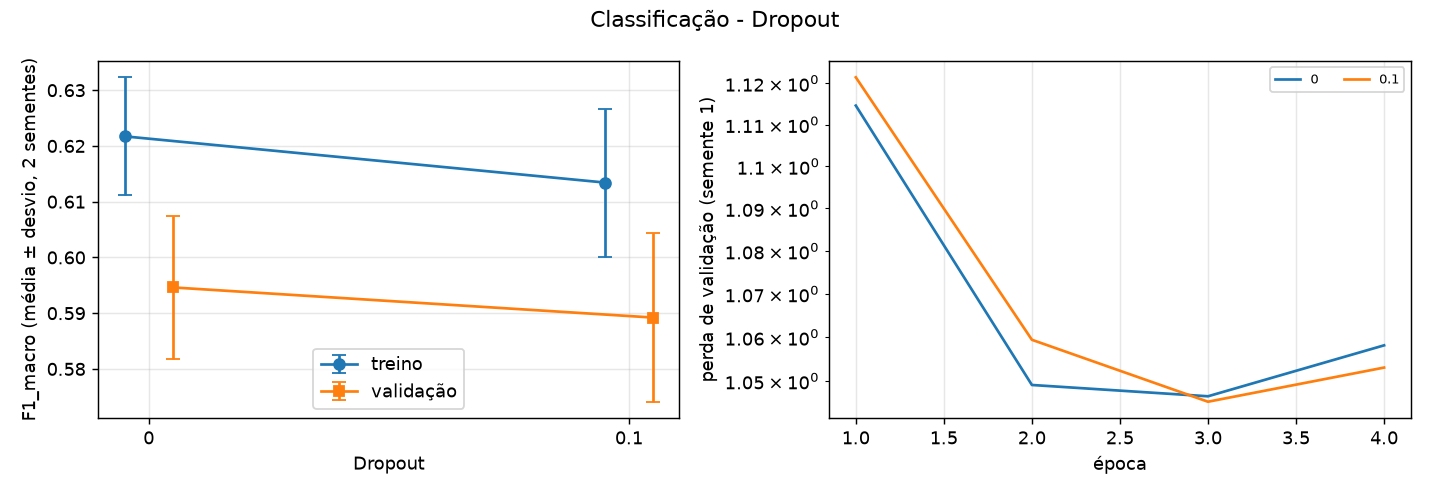
\includegraphics[width=0.95\linewidth]{hp_clf_dropout}\caption{Dropout -- classificação: métrica final por valor (esq.) e perda de validação por época (dir., semente 1).}\end{figure}
\begin{figure}[H]\centering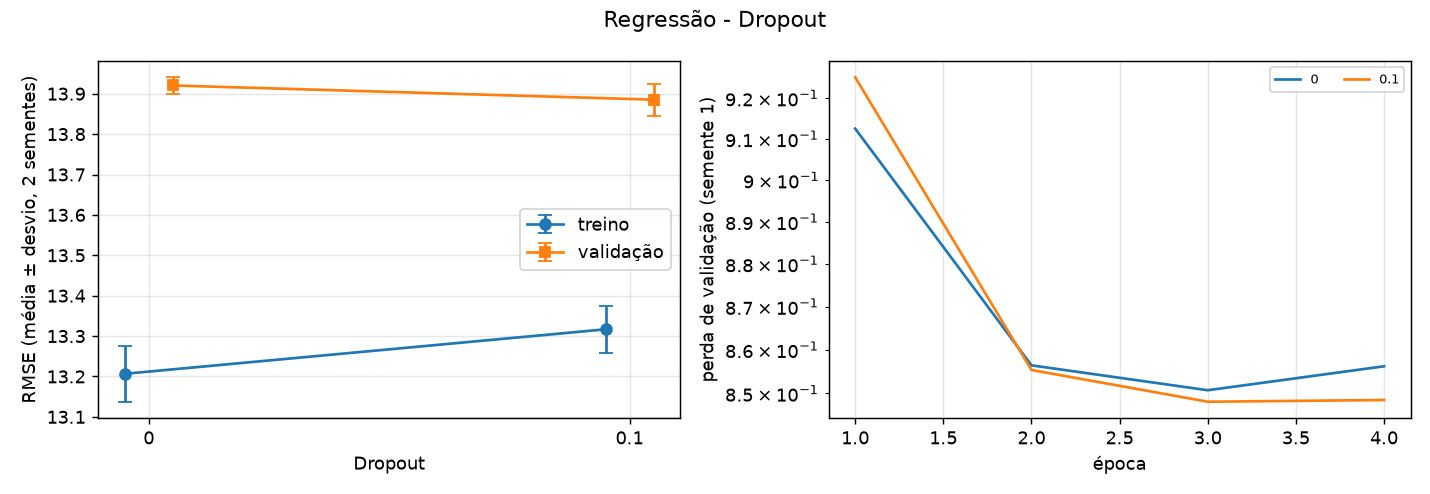
\includegraphics[width=0.95\linewidth]{hp_reg_dropout}\caption{Dropout -- regressão: métrica final por valor (esq.) e perda de validação por época (dir., semente 1).}\end{figure}
\paragraph{(a) Hipótese.} Desligar neurônios aleatoriamente durante o treino é uma regularização estocástica: reduz o desempenho de treino e o gap; em excesso, causa underfitting. Na inferência o dropout é desativado com \texttt{eval()}.

\paragraph{(b) Evidência.} Na classificação, o melhor F1 macro de validação foi 0,595 $\pm$ 0,013 (0) e o pior 0,589 $\pm$ 0,015 (0,1); a diferença de 0,005 é menor que a soma dos desvios (0,028), logo o efeito está dentro do ruído entre sementes e não deve ser tratado como real. O gap variou de 0,024 (0,1) a 0,027 (0). A melhor época média foi de 3 (0) a 3 (0), e o tempo médio de treino de 0,3 s a 0,3 s. Na regressão, o melhor RMSE (mmHg) de validação foi 13,885 $\pm$ 0,040 (0,1) e o pior 13,920 $\pm$ 0,020 (0); a diferença de 0,035 é menor que a soma dos desvios (0,060), logo o efeito está dentro do ruído entre sementes e não deve ser tratado como real. O gap variou de 0,569 (0,1) a 0,714 (0). A melhor época média foi de 3 (0) a 3 (0), e o tempo médio de treino de 0,3 s a 0,3 s.

\paragraph{(c) Mecanismo.} Cada passo treina uma sub-rede diferente, o que impede a coadaptação de neurônios e funciona como um conjunto (ensemble) implícito; o desempenho de treino cai porque a rede é avaliada com ruído durante o ajuste.
% REVISAR: relacione o mecanismo com as curvas acima.

\paragraph{(d) Conclusão prática.} Na classificação, os valores estatisticamente empatados com o melhor (0) foram: 0, 0,1. Do menor (0) para o maior valor (0,1), o desempenho de treino foi de 0,622 para 0,613 e o gap de 0,027 para 0,024: a hipótese de redução da variância se confirmou (diagnóstico com o maior valor: bem ajustado). Na regressão, os valores estatisticamente empatados com o melhor (0,1) foram: 0, 0,1. Do menor (0) para o maior valor (0,1), o desempenho de treino foi de 13,207 para 13,317 e o gap de 0,714 para 0,569: a hipótese de redução da variância se confirmou (diagnóstico com o maior valor: bem ajustado).
% REVISAR

\subsection{Função de perda}
Valores testados: BCE, BCE\_pos\_weight (classificação) e MSE, MAE (regressão) (opcional).

\begin{table}[H]\centering\scriptsize\resizebox{\ifdim\width>\linewidth\linewidth\else\width\fi}{!}{%
\begin{tabular}{lrrrrrrr}\toprule
valor & parâm. & F1 macro treino & F1 macro validação & gap & época parada & tempo (s) & diagnóstico \\\midrule
BCE & 3137 & 0,465 $\pm$ 0,004 & 0,464 $\pm$ 0,015 & 0,001 & 3,5 & 0,3 & underfitting \\
BCE\_pos\_weight & 3137 & 0,622 $\pm$ 0,011 & 0,595 $\pm$ 0,013 & 0,027 & 3,0 & 0,3 & bem ajustado \\
\bottomrule\end{tabular}}
\caption{Função de perda -- classificação (média $\pm$ desvio entre 2 sementes; gap = treino $-$ validação).}\label{tab:clf_loss}\end{table}
\begin{table}[H]\centering\scriptsize\resizebox{\ifdim\width>\linewidth\linewidth\else\width\fi}{!}{%
\begin{tabular}{lrrrrrrr}\toprule
valor & parâm. & RMSE (mmHg) treino & RMSE (mmHg) validação & gap & época parada & tempo (s) & diagnóstico \\\midrule
MSE & 3265 & 13,207 $\pm$ 0,069 & 13,920 $\pm$ 0,020 & 0,714 & 3,0 & 0,3 & bem ajustado \\
MAE & 3265 & 13,356 $\pm$ 0,060 & 13,908 $\pm$ 0,014 & 0,552 & 3,0 & 0,3 & bem ajustado \\
\bottomrule\end{tabular}}
\caption{Função de perda -- regressão (média $\pm$ desvio entre 2 sementes; gap = treino $-$ validação em erro: validação $-$ treino).}\label{tab:reg_loss}\end{table}
\begin{figure}[H]\centering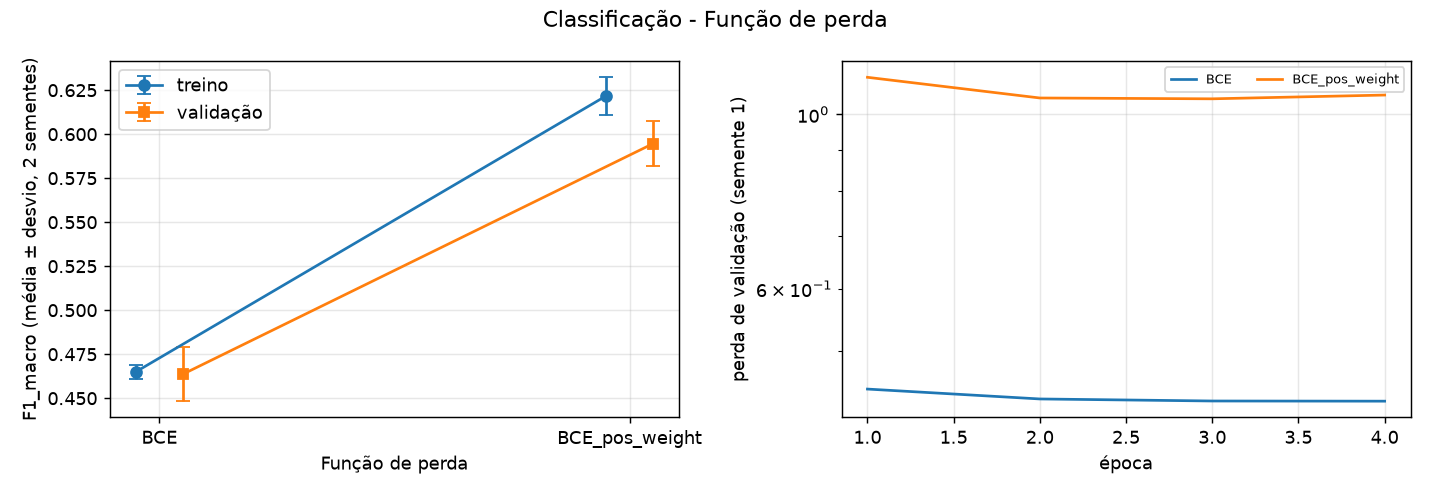
\includegraphics[width=0.95\linewidth]{hp_clf_loss}\caption{Função de perda -- classificação: métrica final por valor (esq.) e perda de validação por época (dir., semente 1).}\end{figure}
\begin{figure}[H]\centering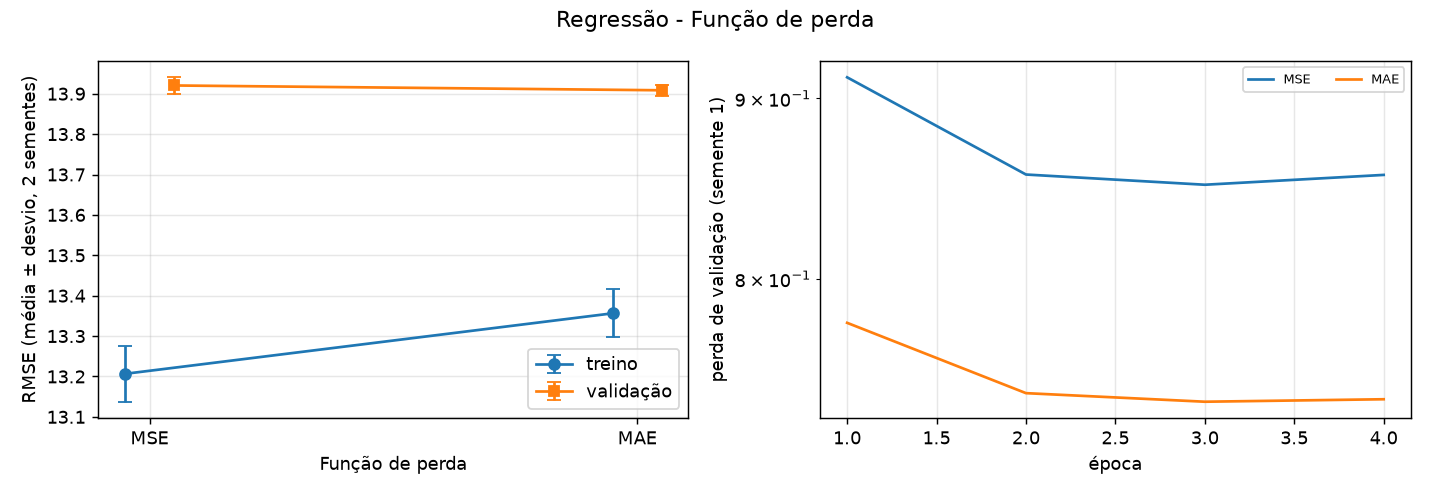
\includegraphics[width=0.95\linewidth]{hp_reg_loss}\caption{Função de perda -- regressão: métrica final por valor (esq.) e perda de validação por época (dir., semente 1).}\end{figure}
\paragraph{(a) Hipótese.} Regressão: MSE penaliza resíduos grandes quadraticamente (sensível a outliers), MAE linearmente e Huber combina os dois. Classificação: com 17\% de positivos, a BCE sem peso tende a prever a classe majoritária; \texttt{pos\_weight} $= n_{neg}/n_{pos}$ equilibra o gradiente das duas classes.

\paragraph{(b) Evidência.} Na classificação, o melhor F1 macro de validação foi 0,595 $\pm$ 0,013 (BCE\_pos\_weight) e o pior 0,464 $\pm$ 0,015 (BCE); a diferença de 0,131 é maior que a soma dos desvios (0,028), logo o efeito é real. O gap variou de 0,001 (BCE) a 0,027 (BCE\_pos\_weight). A melhor época média foi de 3 (BCE\_pos\_weight) a 4 (BCE), e o tempo médio de treino de 0,3 s a 0,3 s. Na regressão, o melhor RMSE (mmHg) de validação foi 13,908 $\pm$ 0,014 (MAE) e o pior 13,920 $\pm$ 0,020 (MSE); a diferença de 0,012 é menor que a soma dos desvios (0,034), logo o efeito está dentro do ruído entre sementes e não deve ser tratado como real. O gap variou de 0,552 (MAE) a 0,714 (MSE). A melhor época média foi de 3 (MSE) a 3 (MSE), e o tempo médio de treino de 0,3 s a 0,3 s.

\paragraph{(c) Mecanismo.} A perda define a direção do gradiente: no MSE, o gradiente de cada amostra é proporcional ao resíduo; no MAE é constante em módulo; o Huber é quadrático perto de zero e linear longe. Na BCE com \texttt{pos\_weight}, o gradiente das amostras positivas é multiplicado pelo peso.
% REVISAR: relacione o mecanismo com as curvas acima.

\paragraph{(d) Conclusão prática.} Na classificação, os valores estatisticamente empatados com o melhor (BCE\_pos\_weight) foram: BCE\_pos\_weight. Com limiar fixo de 0,5, a BCE sem peso obteve F1 macro 0,464 contra 0,595 com \texttt{pos\_weight}; o peso ajudou a classe minoritária. Na regressão, os valores estatisticamente empatados com o melhor (MAE) foram: MSE, MAE. Como a métrica principal é o RMSE, a perda MSE (que otimiza o mesmo critério) é favorecida; MAE e Huber reduzem o peso dos resíduos grandes (outliers de pressão).
% REVISAR

\subsection{Padronização das features}
Valores testados: 1, 0 (opcional).

\begin{table}[H]\centering\scriptsize\resizebox{\ifdim\width>\linewidth\linewidth\else\width\fi}{!}{%
\begin{tabular}{lrrrrrrr}\toprule
valor & parâm. & F1 macro treino & F1 macro validação & gap & época parada & tempo (s) & diagnóstico \\\midrule
com & 3137 & 0,622 $\pm$ 0,011 & 0,595 $\pm$ 0,013 & 0,027 & 3,0 & 0,3 & bem ajustado \\
sem & 3137 & 0,323 $\pm$ 0,250 & 0,319 $\pm$ 0,244 & 0,004 & 1,0 & 0,2 & underfitting \\
\bottomrule\end{tabular}}
\caption{Padronização das features -- classificação (média $\pm$ desvio entre 2 sementes; gap = treino $-$ validação).}\label{tab:clf_scale}\end{table}
\begin{table}[H]\centering\scriptsize\resizebox{\ifdim\width>\linewidth\linewidth\else\width\fi}{!}{%
\begin{tabular}{lrrrrrrr}\toprule
valor & parâm. & RMSE (mmHg) treino & RMSE (mmHg) validação & gap & época parada & tempo (s) & diagnóstico \\\midrule
com & 3265 & 13,207 $\pm$ 0,069 & 13,920 $\pm$ 0,020 & 0,714 & 3,0 & 0,3 & bem ajustado \\
sem & 3265 & 22,773 $\pm$ 2,801 & 22,897 $\pm$ 2,230 & 0,123 & 4,0 & 0,3 & underfitting \\
\bottomrule\end{tabular}}
\caption{Padronização das features -- regressão (média $\pm$ desvio entre 2 sementes; gap = treino $-$ validação em erro: validação $-$ treino).}\label{tab:reg_scale}\end{table}
\begin{figure}[H]\centering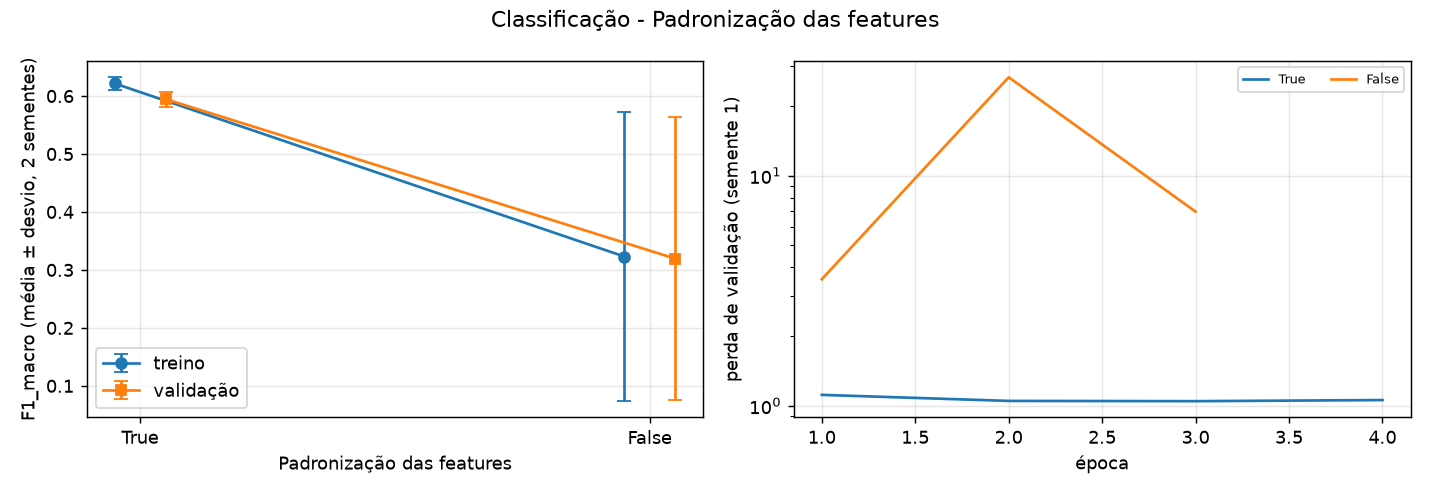
\includegraphics[width=0.95\linewidth]{hp_clf_scale}\caption{Padronização das features -- classificação: métrica final por valor (esq.) e perda de validação por época (dir., semente 1).}\end{figure}
\begin{figure}[H]\centering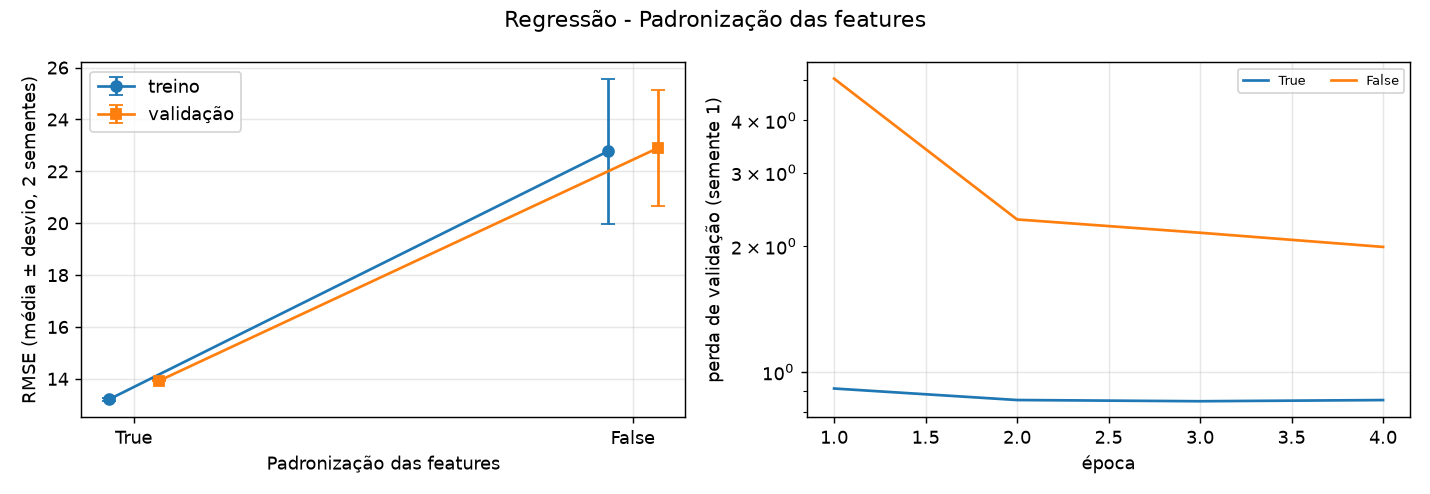
\includegraphics[width=0.95\linewidth]{hp_reg_scale}\caption{Padronização das features -- regressão: métrica final por valor (esq.) e perda de validação por época (dir., semente 1).}\end{figure}
\paragraph{(a) Hipótese.} Sem padronização, features em escalas muito diferentes (ex.: \texttt{Income\_USD} na casa de $10^5$ e variáveis one-hot em $\{0,1\}$) produzem gradientes desbalanceados e saturação, prejudicando ou impedindo o treino.

\paragraph{(b) Evidência.} Na classificação, o melhor F1 macro de validação foi 0,595 $\pm$ 0,013 (com) e o pior 0,319 $\pm$ 0,244 (sem); a diferença de 0,275 é maior que a soma dos desvios (0,257), logo o efeito é real. O gap variou de 0,004 (sem) a 0,027 (com). A melhor época média foi de 1 (sem) a 3 (com), e o tempo médio de treino de 0,2 s a 0,3 s. Na regressão, o melhor RMSE (mmHg) de validação foi 13,920 $\pm$ 0,020 (com) e o pior 22,897 $\pm$ 2,230 (sem); a diferença de 8,976 é maior que a soma dos desvios (2,251), logo o efeito é real. O gap variou de 0,123 (sem) a 0,714 (com). A melhor época média foi de 3 (com) a 4 (sem), e o tempo médio de treino de 0,3 s a 0,3 s.

\paragraph{(c) Mecanismo.} A descida do gradiente usa o mesmo $\eta$ para todos os pesos; features com variância enorme dominam o produto $w^\top x$, saturam as ativações e tornam a superfície de perda mal condicionada.
% REVISAR: relacione o mecanismo com as curvas acima.

\paragraph{(d) Conclusão prática.} Na classificação, os valores estatisticamente empatados com o melhor (com) foram: com. Sem padronização a validação foi 0,319 contra 0,595 com padronização: a hipótese se confirmou. Na regressão, os valores estatisticamente empatados com o melhor (com) foram: com. Sem padronização a validação foi 22,897 contra 13,920 com padronização: a hipótese se confirmou.
% REVISAR



\subsection{Interação entre hiperparâmetros: taxa de aprendizado $\times$ batch}
\begin{table}[H]\centering\scriptsize\resizebox{\ifdim\width>\linewidth\linewidth\else\width\fi}{!}{%
\begin{tabular}{lrr}\toprule
$\eta$ \textbackslash{} batch & 32 & 128 \\\midrule
0,001 & 0,595 $\pm$ 0,013 & 0,580 $\pm$ 0,016 \\
0,01 & 0,612 $\pm$ 0,004 & 0,595 $\pm$ 0,045 \\
\bottomrule\end{tabular}}
\caption{Mapa de calor (classificação): F1 macro de validação, média $\pm$ desvio.}\label{tab:hm_clf}\end{table}
\begin{figure}[H]\centering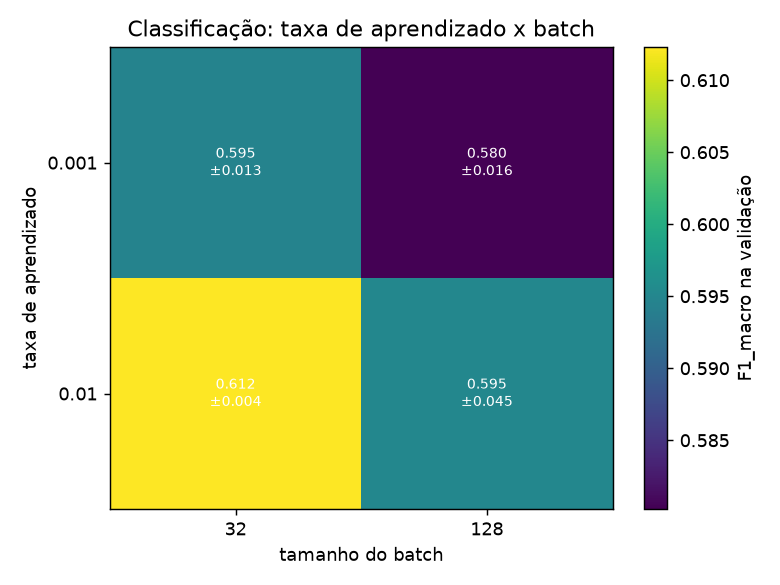
\includegraphics[width=0.6\linewidth]{heatmap_clf}\caption{Interação taxa de aprendizado $\times$ batch -- classificação.}\end{figure}
Na classificação, o melhor $\eta$ para cada batch foi: batch 32: $\eta$ = 0,01 (0,612); batch 128: $\eta$ = 0,01 (0,595). O mesmo $\eta$ foi o melhor para todos os batches; a interação aparece apenas na intensidade do efeito (compare as linhas do mapa), não na posição do ótimo. 

\begin{table}[H]\centering\scriptsize\resizebox{\ifdim\width>\linewidth\linewidth\else\width\fi}{!}{%
\begin{tabular}{lrr}\toprule
$\eta$ \textbackslash{} batch & 32 & 128 \\\midrule
0,001 & 13,920 $\pm$ 0,020 & 14,031 $\pm$ 0,056 \\
0,01 & 13,884 $\pm$ 0,048 & 13,872 $\pm$ 0,029 \\
\bottomrule\end{tabular}}
\caption{Mapa de calor (regressão): RMSE (mmHg) de validação, média $\pm$ desvio.}\label{tab:hm_reg}\end{table}
\begin{figure}[H]\centering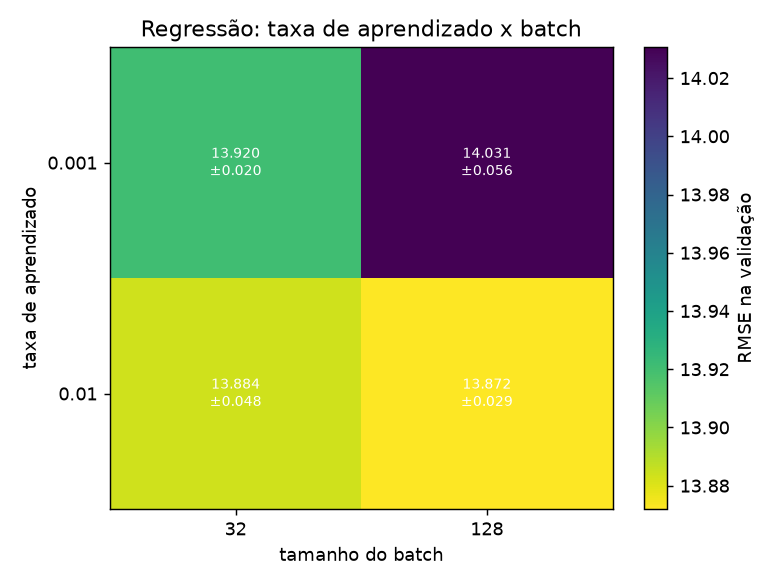
\includegraphics[width=0.6\linewidth]{heatmap_reg}\caption{Interação taxa de aprendizado $\times$ batch -- regressão.}\end{figure}
Na regressão, o melhor $\eta$ para cada batch foi: batch 32: $\eta$ = 0,01 (13,884); batch 128: $\eta$ = 0,01 (13,872). O mesmo $\eta$ foi o melhor para todos os batches; a interação aparece apenas na intensidade do efeito (compare as linhas do mapa), não na posição do ótimo. 



\subsection{Busca final}
Com base nos estudos isolados, fizemos uma busca aleatória com 2 configurações (2 sementes cada) em um espaço
que exclui os valores que divergiram ou foram claramente piores (ex.: $\eta \in [3\cdot10^{-4}, 10^{-2}]$ log-uniforme, sem Sigmoid
e sem SGD simples, 1 a 3 camadas). A escolha usa apenas a média na validação.
\begin{table}[H]\centering\scriptsize\resizebox{\ifdim\width>\linewidth\linewidth\else\width\fi}{!}{%
\begin{tabular}{lrrrrrrrrrr}\toprule
id & neurônios & camadas & ativação & otimizador & $\eta$ & batch & w. decay & dropout & F1 macro val. & gap \\\midrule
0 & 16 & 3 & GELU & AdamW & 6.1e-03 & 32 & 0.0001 & 0 & 0,605 $\pm$ 0,011 & 0,014 \\
1 & 16 & 2 & Tanh & RMSprop & 4.7e-03 & 128 & 0.0001 & 0 & 0,572 $\pm$ 0,004 & 0,026 \\
\bottomrule\end{tabular}}
\caption{Busca aleatória (2 configurações, 2 sementes cada) -- classificação: 8 melhores na validação.}\label{tab:busca_clf}\end{table}
\begin{table}[H]\centering\scriptsize\resizebox{\ifdim\width>\linewidth\linewidth\else\width\fi}{!}{%
\begin{tabular}{lrrrrrrrrrr}\toprule
id & neurônios & camadas & ativação & otimizador & $\eta$ & batch & w. decay & dropout & RMSE (mmHg) val. & gap \\\midrule
1 & 16 & 2 & Tanh & RMSprop & 4.7e-03 & 128 & 0.0001 & 0 & 13,846 $\pm$ 0,017 & 0,444 \\
0 & 16 & 3 & GELU & AdamW & 6.1e-03 & 32 & 0.0001 & 0 & 13,853 $\pm$ 0,034 & 0,454 \\
\bottomrule\end{tabular}}
\caption{Busca aleatória (2 configurações, 2 sementes cada) -- regressão: 8 melhores na validação.}\label{tab:busca_reg}\end{table}

\textbf{Configuração final -- classificação:} 3 camada(s) oculta(s) de 16 neurônios, GELU, AdamW, $\eta$ = 6.1e-03, batch 32, weight decay 0.0001, dropout 0, até 4 épocas com paciência 2; validação 0,605 $\pm$ 0,011.\\
\textbf{Configuração final -- regressão:} 2 camada(s) oculta(s) de 16 neurônios, Tanh, RMSprop, $\eta$ = 4.7e-03, batch 128, weight decay 0.0001, dropout 0, até 4 épocas com paciência 2; validação 13,846 $\pm$ 0,017 mmHg.

\section{Persistência e Inferência}
\subsection{state\_dict $\times$ modelo inteiro}
Há duas formas de salvar uma rede em PyTorch. (i) \texttt{torch.save(modelo.state\_dict(), caminho)} grava só os tensores de pesos e
vieses; para carregar, recria-se a arquitetura (\texttt{MLP(...)}) e chama-se \texttt{load\_state\_dict}. Não depende da estrutura de
pastas do código e pode ser lido com \texttt{torch.load(..., weights\_only=True)}, que só aceita tensores e tipos simples e por isso
não executa código arbitrário. (ii) \texttt{torch.save(modelo, caminho)} serializa o objeto inteiro com \emph{pickle}: fica acoplado
ao nome da classe e ao caminho do módulo (\texttt{src.rn\_models.MLP}), quebra se o código mudar de lugar e exige
\texttt{weights\_only=False}, o que é inseguro com arquivos desconhecidos (um pickle malicioso executa código ao ser carregado).
\textbf{Adotamos o state\_dict}, dentro de um checkpoint completo.
\begin{table}[H]\centering\scriptsize\resizebox{\ifdim\width>\linewidth\linewidth\else\width\fi}{!}{%
\begin{tabular}{lrrrrrr}\toprule
problema & checkpoint (KB) & modelo inteiro (KB) & inteiro c/ weights\_only=True & parâmetros & parâm. $\times$ 4 B (KB) & overhead (KB) \\\midrule
classificação & 14,8 & 11,7 & falhou (UnpicklingError) & 1585 & 6,2 & 8,6 \\
regressão & 13,4 & 9,9 & falhou (UnpicklingError) & 1377 & 5,4 & 8,0 \\
\bottomrule\end{tabular}}
\caption{Tamanho em disco e relação com o número de parâmetros (float32). O overhead do checkpoint inclui média/desvio do scaler, nomes das features, codificação das categóricas e metadados do formato.}\label{tab:tam}\end{table}
\subsection{Conteúdo do checkpoint}
Cada arquivo (\texttt{models/modelo\_classificacao.pt} e \texttt{models/modelo\_regressao.pt}) é um dicionário com:
\texttt{state\_dict}; \texttt{arch} (dimensão de entrada, camadas ocultas, ativação, dropout -- para recriar a rede);
\texttt{config\_treino} (todos os hiperparâmetros); \texttt{x\_media} e \texttt{x\_desvio} (StandardScaler ajustado no treino);
\texttt{features} (nomes das colunas na ordem de entrada); \texttt{encoder} (medianas, modas e categorias do treino, para imputar e
codificar amostras novas a partir das colunas originais); \texttt{y\_media}/\texttt{y\_desvio} (target padronizado, regressão);
\texttt{classes} e \texttt{limiar} (classificação). Sem o pré-processamento, o modelo carregado receberia entradas em outra escala e
produziria previsões erradas.

\subsection{Carregamento em ambiente limpo e fidelidade}
O script \texttt{src/inference.py} é executado em um \emph{processo Python separado} (não compartilha nenhuma variável do treino):
carrega o arquivo com \texttt{map\_location="cpu"} e \texttt{weights\_only=True}, recria a arquitetura, aplica o pré-processamento
salvo, chama \texttt{modelo.eval()} e prevê dentro de \texttt{torch.inference\_mode()}. Saída obtida (classificação):
\begin{verbatim}
$ python src/inference.py --modelo models/modelo_classificacao_rapido.pt --entrada data/novas_amostras_clf.csv
modelo: models/modelo_classificacao_rapido.pt | problema: clf | arquitetura: {'in_dim': 63, 'out_dim': 1, 'hidden': [16, 16, 16], 'activation': 'GELU', 'dropout': 0.0}
limiar de decisão (escolhido na validação): 0.63
    prob_Yes Hypertension_previsto
0   0.421183                    No
1   0.401926                    No
2   0.404594                    No
3   0.652073                   Yes
4   0.454222                    No
5   0.322508                    No
6   0.513935                    No
7   0.344785                    No
8   0.504676                    No
\end{verbatim}
\begin{table}[H]\centering\scriptsize\resizebox{\ifdim\width>\linewidth\linewidth\else\width\fi}{!}{%
\begin{tabular}{lrrrrrr}\toprule
problema & modelo & torch.allclose & dif. máx. abs. & métrica antes de salvar & métrica do carregado & idênticas \\\midrule
classificação & Baseline RN & sim & 0.00e+00 & 0,627095 & 0,627095 & sim \\
classificação & RN final & sim & 0.00e+00 & 0,623221 & 0,623221 & sim \\
classificação & processo separado (20 amostras) & -- & 4.82e-08 & -- & -- & -- \\
regressão & Baseline RN & sim & 0.00e+00 & 13,863369 & 13,863369 & sim \\
regressão & RN final & sim & 0.00e+00 & 13,797115 & 13,797115 & sim \\
regressão & processo separado (20 amostras) & -- & 8.54e-06 & -- & -- & -- \\
\bottomrule\end{tabular}}
\caption{Verificação de fidelidade no teste: saídas do modelo em memória $\times$ modelo carregado do .pt (métrica principal).}\label{tab:fid}\end{table}
\paragraph{E se esquecer o \texttt{eval()}?} Em modo de treino o dropout continua sorteando neurônios a cada chamada: a mesma
entrada gera saídas diferentes e o desempenho cai, porque a rede é avaliada com ruído (e, se houvesse BatchNorm, usaria as estatísticas
do lote em vez das acumuladas). \texttt{eval()} desliga o dropout; \texttt{torch.no\_grad()}/\texttt{inference\_mode()} apenas evitam
guardar o grafo do autograd (menos memória e tempo), não substituem o \texttt{eval()}.
\begin{table}[H]\centering\scriptsize\resizebox{\ifdim\width>\linewidth\linewidth\else\width\fi}{!}{%
\begin{tabular}{lrrrr}\toprule
problema & modelo usado & com eval() & sem eval() (5 passadas) & dif. máx. entre 2 passadas \\\midrule
classificação & configuração final com dropout = 0,3 (o modelo final não tem dropout) & 0,590 & 0,588 $\pm$ 0,003 & 2.070 \\
regressão & configuração final com dropout = 0,3 (o modelo final não tem dropout) & 13,855 & 14,016 $\pm$ 0,032 & 0.663 \\
\bottomrule\end{tabular}}
\caption{Efeito de esquecer \texttt{eval()} (métrica principal na validação).}\label{tab:eval}\end{table}
\paragraph{Portabilidade.} O treino foi feito em CPU. Se fosse feito em GPU, os tensores do \texttt{state\_dict} ficariam
salvos como tensores CUDA; \texttt{map\_location="cpu"} os remapeia para a CPU ao carregar, permitindo usar o modelo em uma máquina sem
GPU (sem ele, o carregamento falha com erro de dispositivo CUDA).

\begin{table}[H]\centering\scriptsize\resizebox{\ifdim\width>\linewidth\linewidth\else\width\fi}{!}{%
\begin{tabular}{lrrrrr}\toprule
problema & versão & disco (KB) & ms/amostra (lote) & amostras/s & métrica principal (teste) \\\midrule
classificação & torchscript & 20,6 & 0,00013 & 7791277 & 0,623 \\
classificação & quantizado\_int8 & 7,7 & 0,00022 & 4642094 & 0,623 \\
classificação & original & 14,8 & 0,00013 & 7495428 & 0,623 \\
regressão & torchscript & 16,9 & 0,00011 & 9022909 & 13,797 \\
regressão & quantizado\_int8 & 6,3 & 0,00025 & 4046628 & 13,792 \\
regressão & original & 13,4 & 0,00015 & 6852804 & 13,797 \\
\bottomrule\end{tabular}}
\caption{Desafio opcional: TorchScript (\texttt{torch.jit.trace}) e quantização dinâmica int8 (\texttt{quantize\_dynamic}).}\label{tab:extras}\end{table}


\section{Resultados}
\subsection{Desempenho -- classificação}
\begin{table}[H]\centering\scriptsize\resizebox{\ifdim\width>\linewidth\linewidth\else\width\fi}{!}{%
\begin{tabular}{llrrrrrrrrr}\toprule
modelo & conjunto & Accuracy & Precision\_macro & Recall\_macro & F1\_macro & Precision\_pos & Recall\_pos & F1\_pos & ROC\_AUC & PR\_AUC \\\midrule
Baseline RN & treino & 0,823 & 0,684 & 0,669 & 0,676 & 0,484 & 0,435 & 0,458 & 0,756 & 0,407 \\
Baseline RN & validacao & 0,833 & 0,702 & 0,678 & 0,688 & 0,517 & 0,442 & 0,477 & 0,700 & 0,410 \\
Baseline RN & teste & 0,797 & 0,634 & 0,622 & 0,627 & 0,399 & 0,355 & 0,375 & 0,673 & 0,338 \\
RN final & treino & 0,789 & 0,639 & 0,651 & 0,644 & 0,397 & 0,440 & 0,418 & 0,730 & 0,368 \\
RN final & validacao & 0,799 & 0,662 & 0,686 & 0,672 & 0,430 & 0,514 & 0,469 & 0,709 & 0,398 \\
RN final & teste & 0,779 & 0,620 & 0,627 & 0,623 & 0,368 & 0,395 & 0,381 & 0,675 & 0,340 \\
\bottomrule\end{tabular}}
\caption{Métricas da Aula 08 (classificação), calculadas com o modelo \emph{carregado do arquivo .pt}. \emph{pos} = classe Yes; limiar escolhido na validação.}\label{tab:met_clf}\end{table}
\begin{figure}[H]\centering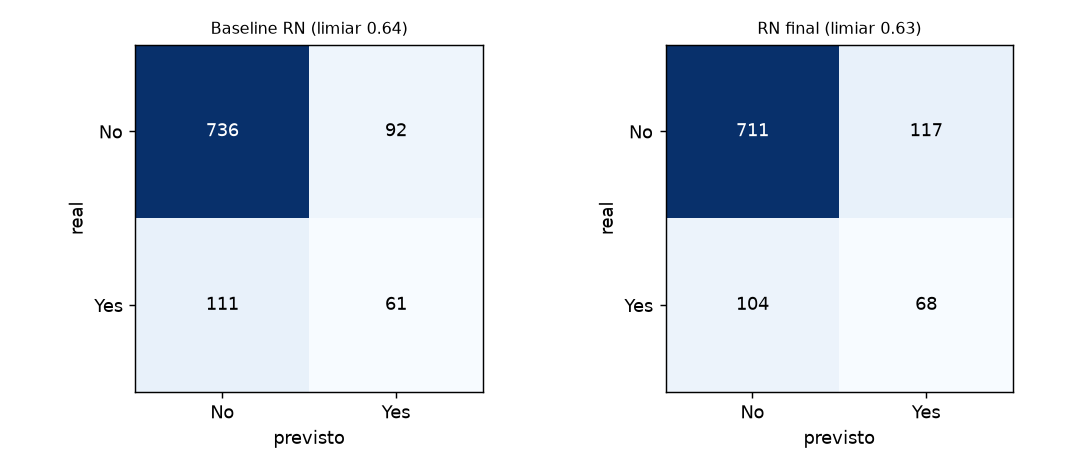
\includegraphics[width=0.75\linewidth]{matrizes_confusao_clf}\caption{Matrizes de confusão no teste.}\end{figure}
\begin{figure}[H]\centering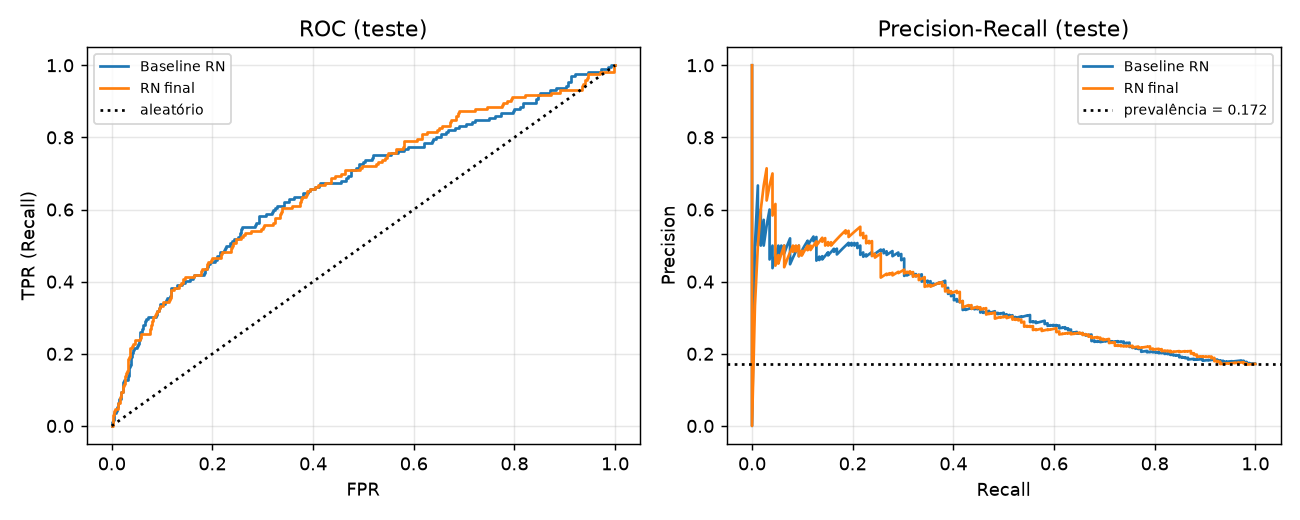
\includegraphics[width=0.95\linewidth]{roc_pr_clf}\caption{Curvas ROC e Precision-Recall no teste (probabilidades da rede, \texttt{torch.sigmoid}).}\end{figure}
\begin{figure}[H]\centering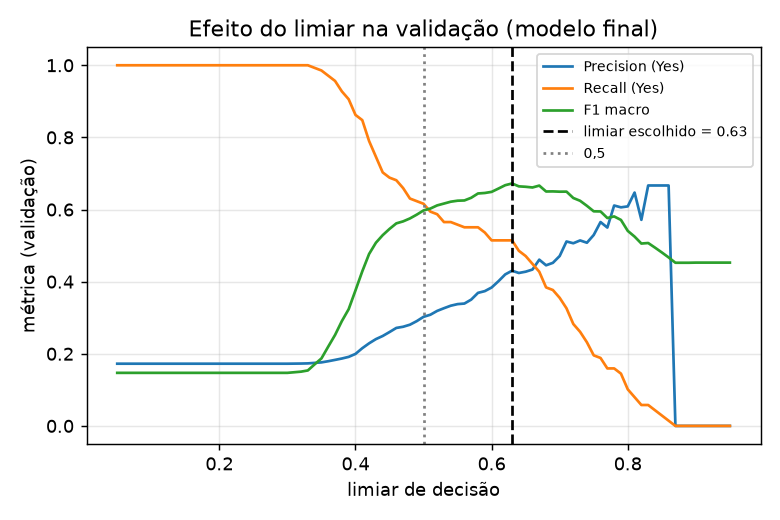
\includegraphics[width=0.6\linewidth]{limiar_clf}\caption{Precision, Recall e F1 macro em função do limiar, na validação (modelo final).}\end{figure}
\paragraph{Limiar de decisão.} O limiar foi escolhido na \emph{validação}, maximizando o F1 macro: 0,63 no modelo final e 0,64 no baseline. Na validação, com limiar 0,5 a Precision/Recall da classe Yes foram 0,302/0,616, e com o limiar escolhido 0,430/0,514: subir o limiar troca Recall por Precision. Como só 17,2\% dos casos são positivos, um classificador que sempre responde \emph{No} já teria Accuracy de 0,828, sem detectar nenhum hipertenso; por isso a Accuracy é enganosa aqui. \textbf{Métrica principal:} F1 macro (equilibra as duas classes), acompanhada de Recall da classe Yes, já que um falso negativo (hipertenso não identificado) custa mais que um falso positivo (que só gera um exame de confirmação). ROC-AUC e PR-AUC no teste: 0,675 e 0,340 (PR-AUC de um classificador aleatório = prevalência $\approx$ 0,172).

\subsection{Generalização -- classificação}
\begin{table}[H]\centering\scriptsize\resizebox{\ifdim\width>\linewidth\linewidth\else\width\fi}{!}{%
\begin{tabular}{lrrrrrrr}\toprule
modelo & treino & validação & teste & gap & gap rel. & época parada & diagnóstico \\\midrule
Baseline RN & 0,676 & 0,688 & 0,627 & 0,049 & 7,2\% & 3 & bem ajustado \\
RN final & 0,644 & 0,672 & 0,623 & 0,021 & 3,3\% & 1 & bem ajustado \\
\bottomrule\end{tabular}}
\caption{F1 macro e gap de generalização (gap = treino $-$ teste). Overfitting se gap relativo $>$ 10\%; underfitting se o treino fica a menos de 0,05 do modelo constante.}\label{tab:gen_clf}\end{table}
\begin{figure}[H]\centering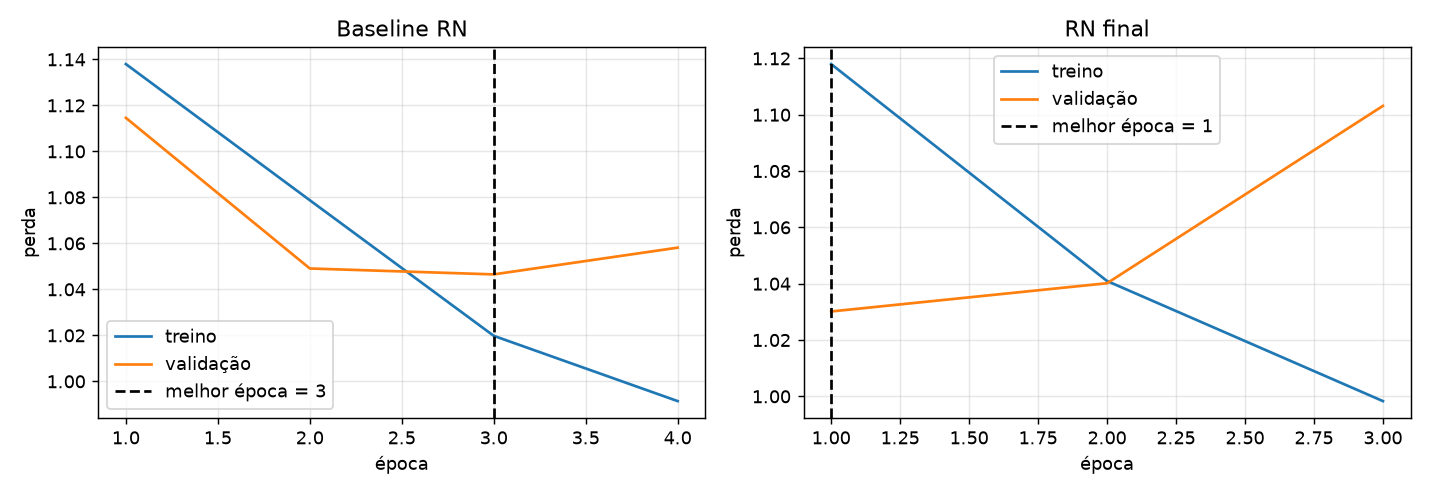
\includegraphics[width=0.95\linewidth]{curvas_aprendizado_clf}\caption{Curvas de aprendizado (perda por época) e ponto do early stopping -- classificação.}\end{figure}
\begin{table}[H]\centering\scriptsize\resizebox{\ifdim\width>\linewidth\linewidth\else\width\fi}{!}{%
\begin{tabular}{lrrr}\toprule
fold & F1\_macro & ROC\_AUC & PR\_AUC \\\midrule
1 & 0,601 & 0,660 & 0,319 \\
2 & 0,594 & 0,640 & 0,295 \\
média $\pm$ desvio & 0,597 $\pm$ 0,005 & 0,650 $\pm$ 0,014 & 0,307 $\pm$ 0,017 \\
\bottomrule\end{tabular}}
\caption{Validação cruzada 2-fold da configuração final no conjunto de treino (classificação).}\label{tab:cv_clf}\end{table}
\begin{table}[H]\centering\scriptsize\resizebox{\ifdim\width>\linewidth\linewidth\else\width\fi}{!}{%
\begin{tabular}{lrrrrr}\toprule
hiperparâmetro & valor & treino & validação & gap & diagnóstico \\\midrule
Neurônios por camada & 2 & 0,453 $\pm$ 0,000 & 0,453 $\pm$ 0,000 & 0,000 & underfitting \\
Neurônios por camada & 4 & 0,547 $\pm$ 0,078 & 0,535 $\pm$ 0,106 & 0,012 & bem ajustado \\
Camadas ocultas & 1 & 0,610 $\pm$ 0,019 & 0,577 $\pm$ 0,018 & 0,033 & bem ajustado \\
Camadas ocultas & 2 & 0,622 $\pm$ 0,011 & 0,595 $\pm$ 0,013 & 0,027 & bem ajustado \\
Taxa de aprendizado & 0,0001 & 0,528 $\pm$ 0,077 & 0,526 $\pm$ 0,080 & 0,002 & bem ajustado \\
Taxa de aprendizado & 0,001 & 0,622 $\pm$ 0,011 & 0,595 $\pm$ 0,013 & 0,027 & bem ajustado \\
Weight decay (L2) & 0 & 0,622 $\pm$ 0,011 & 0,595 $\pm$ 0,013 & 0,027 & bem ajustado \\
Weight decay (L2) & 1e-05 & 0,622 $\pm$ 0,009 & 0,594 $\pm$ 0,012 & 0,028 & bem ajustado \\
Dropout & 0 & 0,622 $\pm$ 0,011 & 0,595 $\pm$ 0,013 & 0,027 & bem ajustado \\
Dropout & 0,1 & 0,613 $\pm$ 0,013 & 0,589 $\pm$ 0,015 & 0,024 & bem ajustado \\
\bottomrule\end{tabular}}
\caption{Configurações extremas do estudo (classificação): classificação em under/overfitting.}\label{tab:ext_clf}\end{table}
O modelo final tem gap de 0,021 (3,3\%) e foi classificado como \emph{bem ajustado}; na validação cruzada, F1 macro = 0,597 $\pm$ 0,005. \textbf{Viés e variância:} aumentar neurônios/camadas reduziu o desempenho de treino perdido (menos viés) e, quando o gap cresceu, aumentou a variância; weight decay e dropout fazem o caminho inverso. % REVISAR com os números das Tabelas.

\subsection{Eficiência computacional -- classificação}
\begin{table}[H]\centering\scriptsize\resizebox{\ifdim\width>\linewidth\linewidth\else\width\fi}{!}{%
\begin{tabular}{lrr}\toprule
medida & Baseline RN & RN final \\\midrule
treino (s) & 0,23 & 0,26 \\
épocas & 4 & 3 \\
RAM pico treino (MB) & 571 & 593 \\
inf. lote (ms/amostra) & 0,00009 & 0,00013 \\
vazão lote (amostras/s) & 10867951 & 7980888 \\
inf. individual (ms) & 0,0235 & 0,0681 \\
c/ pré-proc. (ms/amostra) & 0,0075 & 0,0077 \\
parâmetros & 3137 & 1585 \\
MACs/amostra & 3072 & 1536 \\
disco (KB) & 20,1 & 14,8 \\
energia treino (kWh) & 0,0000010 & 0,0000011 \\
CO$_2$ treino (g) & 0,00004 & 0,00005 \\
\bottomrule\end{tabular}}
\caption{Eficiência (classificação). Energia estimada como potência assumida (15 W) $\times$ tempo; CO$_2$ = kWh $\times$ 45,8 g/kWh (fator do Brasil, Aula 08).}\label{tab:ef_clf}\end{table}
A inferência em lote (0,00013 ms/amostra) é muito mais rápida por amostra que a individual (0,0681 ms), pois o custo fixo de cada chamada (despacho do Python e do PyTorch) é dividido entre todas as amostras e a multiplicação de matrizes aproveita a vetorização da CPU.


\subsection{Desempenho -- regressão}
\begin{table}[H]\centering\scriptsize\resizebox{\ifdim\width>\linewidth\linewidth\else\width\fi}{!}{%
\begin{tabular}{llrrrrrr}\toprule
modelo & conjunto & MAE & MSE & RMSE & MAPE\_\% & R2 & MedAE \\\midrule
Baseline RN & treino & 10,509 & 173,126 & 13,158 & 8,690 & 0,242 & 8,928 \\
Baseline RN & validacao & 11,168 & 194,175 & 13,935 & 9,266 & 0,175 & 9,281 \\
Baseline RN & teste & 11,185 & 192,193 & 13,863 & 9,170 & 0,190 & 9,490 \\
RN final & treino & 10,700 & 179,200 & 13,387 & 8,853 & 0,215 & 9,069 \\
RN final & validacao & 11,084 & 192,050 & 13,858 & 9,191 & 0,184 & 9,721 \\
RN final & teste & 11,169 & 190,360 & 13,797 & 9,157 & 0,197 & 9,420 \\
\bottomrule\end{tabular}}
\caption{Métricas da Aula 08 (regressão), calculadas com o modelo \emph{carregado do arquivo .pt}. Erros em mmHg; MAPE em \%.}\label{tab:met_reg}\end{table}
\begin{figure}[H]\centering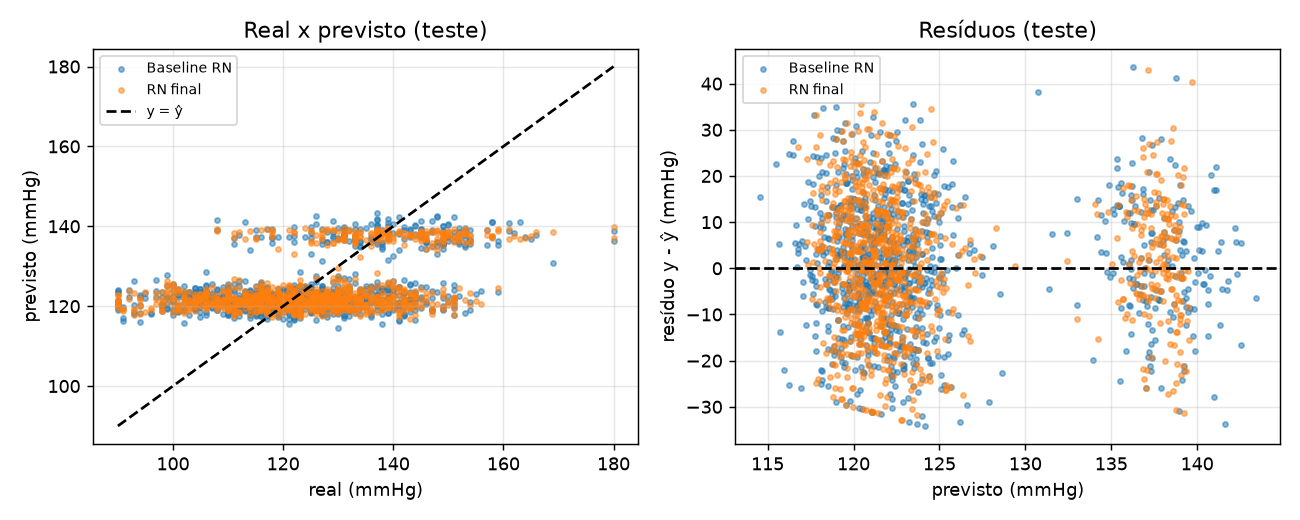
\includegraphics[width=0.95\linewidth]{real_vs_previsto_residuos_reg}\caption{Real $\times$ previsto e resíduos $e_i = y_i - \hat y_i$ no teste, em mmHg.}\end{figure}
\paragraph{Métrica principal e resíduos.} Usamos o RMSE (em mmHg, mesma unidade do target) como métrica principal porque erros grandes de pressão são clinicamente mais graves e o RMSE os penaliza mais; o MAE (11,169 mmHg no teste) é reportado junto por ser menos sensível a outliers. A diferença RMSE $-$ MAE (2,628) indica a presença de resíduos grandes. R$^2$ no teste = 0,197. % REVISAR: descreva o padrão dos resíduos (faixas, viés para valores extremos).

\subsection{Generalização -- regressão}
\begin{table}[H]\centering\scriptsize\resizebox{\ifdim\width>\linewidth\linewidth\else\width\fi}{!}{%
\begin{tabular}{lrrrrrrr}\toprule
modelo & treino & validação & teste & gap & gap rel. & época parada & diagnóstico \\\midrule
Baseline RN & 13,158 & 13,935 & 13,863 & 0,706 & 5,4\% & 3 & bem ajustado \\
RN final & 13,387 & 13,858 & 13,797 & 0,411 & 3,1\% & 4 & bem ajustado \\
\bottomrule\end{tabular}}
\caption{RMSE (mmHg) e gap de generalização (gap = treino $-$ teste; para erro, teste $-$ treino). Overfitting se gap relativo $>$ 10\%; underfitting se o treino fica a menos de 0,05 do modelo constante.}\label{tab:gen_reg}\end{table}
\begin{figure}[H]\centering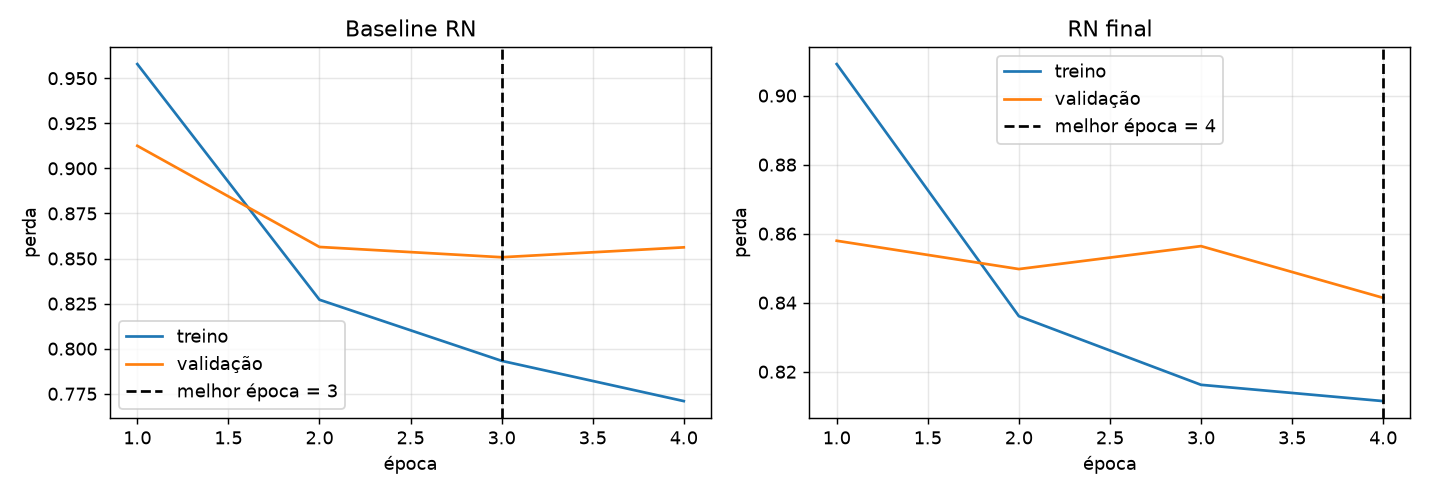
\includegraphics[width=0.95\linewidth]{curvas_aprendizado_reg}\caption{Curvas de aprendizado (perda por época) e ponto do early stopping -- regressão.}\end{figure}
\begin{table}[H]\centering\scriptsize\resizebox{\ifdim\width>\linewidth\linewidth\else\width\fi}{!}{%
\begin{tabular}{lrrr}\toprule
fold & RMSE & MAE & R2 \\\midrule
1 & 13,930 & 11,075 & 0,157 \\
2 & 14,196 & 11,369 & 0,120 \\
média $\pm$ desvio & 14,063 $\pm$ 0,188 & 11,222 $\pm$ 0,208 & 0,139 $\pm$ 0,026 \\
\bottomrule\end{tabular}}
\caption{Validação cruzada 2-fold da configuração final no conjunto de treino (regressão).}\label{tab:cv_reg}\end{table}
\begin{table}[H]\centering\scriptsize\resizebox{\ifdim\width>\linewidth\linewidth\else\width\fi}{!}{%
\begin{tabular}{lrrrrr}\toprule
hiperparâmetro & valor & treino & validação & gap & diagnóstico \\\midrule
Neurônios por camada & 2 & 14,208 $\pm$ 0,700 & 14,444 $\pm$ 0,827 & 0,236 & bem ajustado \\
Neurônios por camada & 4 & 14,790 $\pm$ 0,324 & 15,137 $\pm$ 0,158 & 0,346 & underfitting \\
Camadas ocultas & 1 & 13,280 $\pm$ 0,209 & 13,978 $\pm$ 0,038 & 0,698 & bem ajustado \\
Camadas ocultas & 2 & 13,207 $\pm$ 0,069 & 13,920 $\pm$ 0,020 & 0,714 & bem ajustado \\
Taxa de aprendizado & 0,0001 & 14,794 $\pm$ 0,043 & 15,104 $\pm$ 0,026 & 0,310 & underfitting \\
Taxa de aprendizado & 0,001 & 13,207 $\pm$ 0,069 & 13,920 $\pm$ 0,020 & 0,714 & bem ajustado \\
Weight decay (L2) & 0 & 13,207 $\pm$ 0,069 & 13,920 $\pm$ 0,020 & 0,714 & bem ajustado \\
Weight decay (L2) & 1e-05 & 13,202 $\pm$ 0,070 & 13,916 $\pm$ 0,023 & 0,714 & bem ajustado \\
Dropout & 0 & 13,207 $\pm$ 0,069 & 13,920 $\pm$ 0,020 & 0,714 & bem ajustado \\
Dropout & 0,1 & 13,317 $\pm$ 0,059 & 13,885 $\pm$ 0,040 & 0,569 & bem ajustado \\
\bottomrule\end{tabular}}
\caption{Configurações extremas do estudo (regressão): classificação em under/overfitting.}\label{tab:ext_reg}\end{table}
O modelo final tem gap de 0,411 (3,1\%) e foi classificado como \emph{bem ajustado}; na validação cruzada, RMSE (mmHg) = 14,063 $\pm$ 0,188. \textbf{Viés e variância:} aumentar neurônios/camadas reduziu o desempenho de treino perdido (menos viés) e, quando o gap cresceu, aumentou a variância; weight decay e dropout fazem o caminho inverso. % REVISAR com os números das Tabelas.

\subsection{Eficiência computacional -- regressão}
\begin{table}[H]\centering\scriptsize\resizebox{\ifdim\width>\linewidth\linewidth\else\width\fi}{!}{%
\begin{tabular}{lrr}\toprule
medida & Baseline RN & RN final \\\midrule
treino (s) & 0,26 & 0,09 \\
épocas & 4 & 4 \\
RAM pico treino (MB) & 624 & 625 \\
inf. lote (ms/amostra) & 0,00010 & 0,00009 \\
vazão lote (amostras/s) & 10000167 & 11324601 \\
inf. individual (ms) & 0,0248 & 0,0207 \\
c/ pré-proc. (ms/amostra) & 0,0076 & 0,0071 \\
parâmetros & 3265 & 1377 \\
MACs/amostra & 3200 & 1344 \\
disco (KB) & 20,8 & 13,4 \\
energia treino (kWh) & 0,0000011 & 0,0000004 \\
CO$_2$ treino (g) & 0,00005 & 0,00002 \\
\bottomrule\end{tabular}}
\caption{Eficiência (regressão). Energia estimada como potência assumida (15 W) $\times$ tempo; CO$_2$ = kWh $\times$ 45,8 g/kWh (fator do Brasil, Aula 08).}\label{tab:ef_reg}\end{table}
A inferência em lote (0,00009 ms/amostra) é muito mais rápida por amostra que a individual (0,0207 ms), pois o custo fixo de cada chamada (despacho do Python e do PyTorch) é dividido entre todas as amostras e a multiplicação de matrizes aproveita a vetorização da CPU.


\subsection{Efeito dos hiperparâmetros no custo e implantação}
Na classificação: de 2 para 4 neurônios, os parâmetros foram de 137 para 281 (arquivo $\approx$ parâmetros $\times$ 4 bytes) e o tempo médio de 0,3 s para 0,3 s; de 1 para 2 camadas, de 2081 para 3137 parâmetros; o batch não altera os parâmetros, mas o tempo foi de 0,9 s (batch 8) a 0,3 s (32). Na regressão: de 2 para 4 neurônios, os parâmetros foram de 145 para 297 (arquivo $\approx$ parâmetros $\times$ 4 bytes) e o tempo médio de 0,2 s para 0,2 s; de 1 para 2 camadas, de 2209 para 3265 parâmetros; o batch não altera os parâmetros, mas o tempo foi de 0,8 s (batch 8) a 0,3 s (32). 
As redes finais têm poucos milhares de parâmetros e ocupam dezenas de KB: cabem com folga em um dispositivo de borda (ex.: Raspberry Pi
ou microcontrolador com alguns MB de RAM). Para reduzir ainda mais, é possível usar menos neurônios (o estudo mostra que a capacidade
extra rende pouco), quantização int8 (Tabela~\ref{tab:extras}) e poda de pesos pequenos. % REVISAR

\section{Análise e Discussão}
\begin{table}[H]\centering\scriptsize\resizebox{\ifdim\width>\linewidth\linewidth\else\width\fi}{!}{%
\begin{tabular}{lrrrrrrrrrrr}\toprule
problema & modelo & treino & validação & teste & gap & diagnóstico & K-fold & parâm. & treino (s) & ms/amostra & KB \\\midrule
classificação & Baseline RN & 0,676 & 0,688 & 0,627 & 0,049 & bem ajustado & -- & 3137 & 0,2 & 0,00009 & 20,1 \\
classificação & RN final & 0,644 & 0,672 & 0,623 & 0,021 & bem ajustado & 0,597 $\pm$ 0,005 & 1585 & 0,3 & 0,00013 & 14,8 \\
regressão & Baseline RN & 13,158 & 13,935 & 13,863 & 0,706 & bem ajustado & -- & 3265 & 0,3 & 0,00010 & 20,8 \\
regressão & RN final & 13,387 & 13,858 & 13,797 & 0,411 & bem ajustado & 14,063 $\pm$ 0,188 & 1377 & 0,1 & 0,00009 & 13,4 \\
\bottomrule\end{tabular}}
\caption{Tabela-resumo final (métrica principal: F1 macro na classificação, RMSE em mmHg na regressão). Arquivo: \texttt{reports/tables/rn/resumo\_final.csv}.}\label{tab:resumo}\end{table}

\begin{table}[H]\centering\scriptsize\resizebox{\ifdim\width>\linewidth\linewidth\else\width\fi}{!}{%
\begin{tabular}{lrrrrrrrr}\toprule
problema & hiperparâmetro & melhor & val. & pior & val. & amplitude & soma desvios & efeito real \\\midrule
classificação & Padronização das features & com & 0,595 & sem & 0,319 & 0,275 & 0,257 & sim \\
classificação & Função de perda & BCE\_pos\_weight & 0,595 & BCE & 0,464 & 0,131 & 0,028 & sim \\
classificação & Otimizador & SGD\_momentum & 0,534 & SGD & 0,417 & 0,118 & 0,177 & não \\
classificação & Neurônios por camada & 4 & 0,535 & 2 & 0,453 & 0,083 & 0,106 & não \\
classificação & Taxa de aprendizado & 0,001 & 0,595 & 0,0001 & 0,526 & 0,069 & 0,093 & não \\
classificação & Camadas ocultas & 2 & 0,595 & 1 & 0,577 & 0,018 & 0,031 & não \\
classificação & Tamanho do batch & 32 & 0,595 & 8 & 0,582 & 0,013 & 0,018 & não \\
classificação & Dropout & 0 & 0,595 & 0,1 & 0,589 & 0,005 & 0,028 & não \\
classificação & Função de ativação & ReLU & 0,595 & LeakyReLU & 0,593 & 0,001 & 0,028 & não \\
classificação & Weight decay (L2) & 0 & 0,595 & 1e-05 & 0,594 & 0,001 & 0,025 & não \\
regressão & Padronização das features & com & 13,920 & sem & 22,897 & 8,976 & 2,251 & sim \\
regressão & Taxa de aprendizado & 0,001 & 13,920 & 0,0001 & 15,104 & 1,183 & 0,046 & sim \\
regressão & Otimizador & SGD\_momentum & 14,183 & SGD & 15,360 & 1,176 & 0,101 & sim \\
regressão & Neurônios por camada & 2 & 14,444 & 4 & 15,137 & 0,693 & 0,984 & não \\
regressão & Camadas ocultas & 2 & 13,920 & 1 & 13,978 & 0,057 & 0,058 & não \\
regressão & Tamanho do batch & 8 & 13,874 & 32 & 13,920 & 0,046 & 0,038 & sim \\
regressão & Dropout & 0,1 & 13,885 & 0 & 13,920 & 0,035 & 0,060 & não \\
regressão & Função de ativação & LeakyReLU & 13,908 & ReLU & 13,920 & 0,012 & 0,042 & não \\
regressão & Função de perda & MAE & 13,908 & MSE & 13,920 & 0,012 & 0,034 & não \\
regressão & Weight decay (L2) & 1e-05 & 13,916 & 0 & 13,920 & 0,004 & 0,043 & não \\
\bottomrule\end{tabular}}
\caption{Sensibilidade: hiperparâmetros ordenados pelo impacto na validação (melhor $-$ pior valor testado).}\label{tab:sens}\end{table}

\subsection{Respostas -- classificação}
\begin{enumerate}[label=(\alph*)]
\item Padronização das features (amplitude 0,275, efeito real); Função de perda (amplitude 0,131, efeito real); Otimizador (amplitude 0,118, dentro do ruído). Os mecanismos estão na Seção~\ref{sec:hp}. Hiperparâmetros com efeito desprezível (dentro do desvio entre sementes): Otimizador, Neurônios por camada, Taxa de aprendizado, Camadas ocultas, Tamanho do batch, Dropout, Função de ativação, Weight decay (L2). % REVISAR
\item Ver Tabela~\ref{tab:hm_clf} e o texto que a acompanha.
\item F1 macro treino/validação/teste = 0,644/0,672/0,623; gap = 0,021 (3,3\%), diagnóstico: \emph{bem ajustado}; K-fold: 0,597 $\pm$ 0,005.
\item Sim: diferença máxima absoluta entre as saídas = 0.00e+00 (\texttt{torch.allclose} = True). Cuidados: salvar média/desvio do scaler (e do target), a codificação das categóricas e a ordem das features; recriar a mesma arquitetura a partir de \texttt{arch}; chamar \texttt{eval()}; usar \texttt{map\_location} e \texttt{weights\_only=True}.
\item 1585 parâmetros, 1536 MACs por amostra, 14,8 KB em disco, 0,3 s de treino e 0,00013 ms por amostra em lote: custo desprezível para uso em clínica, em servidor ou em dispositivo de borda. % REVISAR conforme o contexto do cliente
\item No teste, a rede final obteve F1 macro = 0,623, contra 0,682 do melhor modelo da atividade anterior (Random Forest). A rede não superou os modelos anteriores, com diferença de 0,059; como árvores e ensembles são mais simples de ajustar e de interpretar, \textbf{não recomendamos} a rede para este problema. % REVISAR
\end{enumerate}

\subsection{Respostas -- regressão}
\begin{enumerate}[label=(\alph*)]
\item Padronização das features (amplitude 8,976, efeito real); Taxa de aprendizado (amplitude 1,183, efeito real); Otimizador (amplitude 1,176, efeito real). Os mecanismos estão na Seção~\ref{sec:hp}. Hiperparâmetros com efeito desprezível (dentro do desvio entre sementes): Neurônios por camada, Camadas ocultas, Dropout, Função de ativação, Função de perda, Weight decay (L2). % REVISAR
\item Ver Tabela~\ref{tab:hm_reg} e o texto que a acompanha.
\item RMSE (mmHg) treino/validação/teste = 13,387/13,858/13,797; gap = 0,411 (3,1\%), diagnóstico: \emph{bem ajustado}; K-fold: 14,063 $\pm$ 0,188.
\item Sim: diferença máxima absoluta entre as saídas = 0.00e+00 (\texttt{torch.allclose} = True). Cuidados: salvar média/desvio do scaler (e do target), a codificação das categóricas e a ordem das features; recriar a mesma arquitetura a partir de \texttt{arch}; chamar \texttt{eval()}; usar \texttt{map\_location} e \texttt{weights\_only=True}.
\item 1377 parâmetros, 1344 MACs por amostra, 13,4 KB em disco, 0,1 s de treino e 0,00009 ms por amostra em lote: custo desprezível para uso em clínica, em servidor ou em dispositivo de borda. % REVISAR conforme o contexto do cliente
\item No teste, a rede final obteve RMSE (mmHg) = 13,797, contra 13,739 do melhor modelo da atividade anterior (Gradient Boosting). A rede não superou os modelos anteriores, com diferença de 0,058; como árvores e ensembles são mais simples de ajustar e de interpretar, \textbf{não recomendamos} a rede para este problema. % REVISAR
\end{enumerate}

\subsection{Comparação com a atividade anterior}
\begin{table}[H]\centering\scriptsize\resizebox{\ifdim\width>\linewidth\linewidth\else\width\fi}{!}{%
\begin{tabular}{lrrrrrr}\toprule
modelo & F1\_macro & ROC\_AUC & PR\_AUC & Accuracy & treino\_tempo\_medio\_s & tamanho\_disco\_kb \\\midrule
Árvore (ajustada) & 0,682 & 0,674 & 0,318 & 0,825 & 0,066 & 9,020 \\
Random Forest & 0,682 & 0,682 & 0,370 & 0,824 & 1,664 & 3703,261 \\
Gradient Boosting & 0,606 & 0,685 & 0,387 & 0,830 & 1,407 & 252,169 \\
Baseline RN & 0,627 & 0,673 & 0,338 & 0,797 & 0,234 & 20,126 \\
RN final & 0,623 & 0,675 & 0,340 & 0,779 & 0,262 & 14,755 \\
\bottomrule\end{tabular}}
\caption{Teste (classificação): modelos da atividade anterior $\times$ redes neurais, mesmos conjuntos de treino e teste. Tempos medidos em execuções diferentes.}\label{tab:comp_clf}\end{table}
\begin{table}[H]\centering\scriptsize\resizebox{\ifdim\width>\linewidth\linewidth\else\width\fi}{!}{%
\begin{tabular}{lrrrrrr}\toprule
modelo & RMSE & MAE & R2 & MAPE\_\% & treino\_tempo\_medio\_s & tamanho\_disco\_kb \\\midrule
Árvore (ajustada) & 13,748 & 11,111 & 0,203 & 9,106 & 0,057 & 9,887 \\
Random Forest & 13,798 & 11,161 & 0,197 & 9,146 & 0,984 & 4308,862 \\
Gradient Boosting & 13,739 & 11,095 & 0,204 & 9,094 & 0,941 & 90,388 \\
Baseline RN & 13,863 & 11,185 & 0,190 & 9,170 & 0,265 & 20,759 \\
RN final & 13,797 & 11,169 & 0,197 & 9,157 & 0,087 & 13,419 \\
\bottomrule\end{tabular}}
\caption{Teste (regressão): modelos da atividade anterior $\times$ redes neurais, mesmos conjuntos de treino e teste. Tempos medidos em execuções diferentes.}\label{tab:comp_reg}\end{table}

\subsection{Vantagens e desvantagens das redes neurais para estes dados}
\textbf{Vantagens:} modelam relações não lineares e interações sem que precisemos especificá-las; o mesmo código serve para
regressão e classificação; o modelo final é pequeno e rápido na inferência. \textbf{Desvantagens:} são sensíveis à escala das
features (Seção~\ref{sec:hp}, padronização) e aos hiperparâmetros (taxa de aprendizado e batch mudam o resultado e até causam
divergência); exigem pré-processamento salvo junto com o modelo; são pouco interpretáveis (ao contrário da árvore de decisão e das regras
do sistema especialista); e, em um conjunto tabular pequeno (5000 linhas) e de sinal fraco, não há dados suficientes para a capacidade
extra fazer diferença.

\subsection{Limitações}
Conjunto sintético e pequeno, com sinal fraco (AUC e R$^2$ baixos para todos os modelos); uma única divisão treino/teste; 2
sementes por configuração; o estudo de um fator por vez não cobre todas as interações (só lr $\times$ batch foi varrido em 2D); a busca
aleatória com 2 configurações é limitada; o limiar 0,5 no estudo de hiperparâmetros (o limiar ótimo só foi escolhido para o
modelo final); a energia foi estimada por potência assumida (15 W), não medida; os tempos dependem do hardware.

\section{Considerações Finais}
\textbf{TODO (aluno):} dificuldades encontradas, o que aprendeu sobre hiperparâmetros e sobre salvar/carregar modelos.

\section{Referência ao Repositório}
Código: \url{https://github.com/xonazz/IA_thomas2}. Estrutura: \texttt{src/rn\_models.py} (classe MLP), \texttt{src/rn\_train.py}
(treino, early stopping, sementes, métricas), \texttt{src/rn\_prep.py} (pré-processamento exportável), \texttt{src/rn\_study.py}
(estudo de hiperparâmetros), \texttt{src/rn\_final.py} (modelo final, persistência, métricas, generalização e eficiência),
\texttt{src/inference.py} (inferência independente), \texttt{src/rn\_report.py} (este relatório), \texttt{run\_rn.py} (executa tudo),
\texttt{models/} (arquivos .pt), \texttt{logs/hiperparametros.csv} (todas as execuções), \texttt{reports/tables/rn} e
\texttt{reports/figures/rn} (tabelas e gráficos) e \texttt{notebooks/rn/} (notebooks 03 a 08).
\end{document}
